\documentclass[12pt,a4paper]{book}
\usepackage[utf8]{inputenc}
\usepackage[english]{babel}
\usepackage{amsmath}
\usepackage{amsfonts}
\usepackage{amssymb}
\usepackage{latexsym}
\usepackage{makeidx}
\usepackage{hyperref}
\usepackage{graphicx}
\usepackage{graphics}
\usepackage{lmodern}
\usepackage{hyperref}
\usepackage{tikz}
\usepackage{subcaption}
\usepackage{dsfont}
\usepackage{multicol}
\usepackage{xcolor}
\usepackage{booktabs}
\usepackage{float}
\usepackage{fancybox}


\definecolor{rojo}{RGB}{255, 0, 0}


\definecolor{rojoclaro}{RGB}{255, 245, 245}

\definecolor{blanco}{RGB}{255, 255, 255}

\definecolor{negro}{RGB}{0, 0, 0}

\definecolor{gris}{RGB}{245, 245, 245}

\newcommand{\R}{\mathbb{R}}
\newcommand{\D}{\mathrm{d}}

\newcommand{\E}{\mathbb{E}}

\newcommand{\EE}[1]{ \mathbb{E} \{ #1 \}  }

\newcommand{\EEE}[1]{\mathbb{E} \left\lbrace #1 \right\rbrace}

\newcommand{\cov}{\mathrm{cov}}

\newcommand{\Par}[1]{\left( #1 \right)}

\newcommand{\integral}{\int_{-\infty}^{\infty}}

\newcommand{\Corchetes}[1]{\left\lbrace #1 \right\rbrace}

\newcommand{\corchetes}[1]{\{ #1 \}}

\newcommand{\parentesis}[1]{\left( #1 \right)}

\newcommand{\parciales}[2]{\frac{\partial #1}{\partial #2}}

\newcommand{\peso}[1]{\sum_{i=1}^n \frac{#1}{\sigma_i^2}}

\newcommand{\suma}[1]{\sum_{i=1}^n  #1}

\newcommand{\chii}{$\chi^2$}

\newcommand{\Nota}[1]{\textcolor{rojo}{\fboxrule=0.4pt \fboxsep=4pt \fcolorbox{rojo}{rojoclaro}{\parbox[][][c]{16.5cm}{\textbf{Nota:} #1}}}} 

\newcommand{\Teorema}[1]{\textcolor{negro}{\fboxrule=0.6pt \fboxsep=6pt \fcolorbox{negro}{blanco}{\parbox[][][c]{16.5cm}{$\bullet \ $ #1}}}} 

\setlength{\parindent}{0px}
\usepackage[left=2cm,right=2cm,top=4cm,bottom=2cm]{geometry}

\author{Daniel Vázquez Lago}
\title{Apuntes de Estadística}

\begin{document}
\maketitle

\newpage

\tableofcontents

\newpage

\chapter*{Introducción}

En este texto trataremos temas como la estadística y probabilidad (partiendo desde lo más básico a conceptos mas complejos) de una manera teórica para luego poder avanzar y entender conceptos mas complicados, que quizá hayáis visto pero su mecanismo teórico es mucho mas profundo del que parece. \\

También analizaremos como hacer memorias, ejemplos de como estructurarlas, que hay que hacer con las incertidumbres, como se usan y combinan, ya que hay una gran falta de información de como proceder en las memorias para expresar correctamente los datos. \\

En general este texto será una introducción relativamente avanzada de como hacer una memoria, que factores hay que tener en cuenta, y cual es la razón teórica para hacer lo que hacemos. 



\chapter{Estadística descriptiva \label{Sec:estadistica}}


En las ciencias experimentales se basan en la contrastación de hipótesis con las medidas empíricas. Cuando se trata de determinar  el valor de una magnitud física es inevitable cierto nivel de variabilidad o imprecisión, que puede venir dada por diversos motivos: imperfección de nuestros instrumentos, la propia fluctuación del mensurando o en la existencia de perturbaciones que no podemos controlar. Es necesario comprender que en cualquier conjunto de medidas de una propiedad física realizadas con instrumentos habrá una inevitable variación entre los valores de las medidas. \\

Supongamos que queremos calcular la masa de un objeto. Para determinarla necesitamos o bien una balanza con una masa patrón o una báscula. Supongamos que usamos una báscula con la precisión suficiente, donde obtenemos: 

$$ m \ (kg)  = \{1.00043; 1.00045; 1.00048; 1.00039; 1.00043 \} $$

Ahora nos podemos hacer las siguientes preguntas: ¿Cuál es el valor que realmente podemos asignar a la masa?¿Coincide con alguno de esos valores?¿Realmente podemos calcular el valor real?¿Con que nivel de certidumbre podemos concluir que conocemos el valor de la masa del cuerpo a partir del experimento anterior? \\

El origen de esta variabilidad en la determinación experimental de las magnitudes físicas es inherente a la naturaleza de los objetos, imputable a las limitaciones de nuestra capacidad de observación (precisión de los instrumentos...). El objeto de este capítulo es la introducción de algunas de las herramientas matemáticas desarrolladas en el ámbito de la Estadística matemática para la descripción de la información contenida en los datos y su posterior utilización para la evaluación de la incertidumbre asociada al proceso experimental. En concreto nos ocuparemos de los conjuntos de datos obtenidos del colectivo objeto de estudio mediante algún experimento (aleatorio) y que posteriormente pretende analizarse. 

\newpage 

\section{Introducción}

En el análisis de una determinada propiedad física debemos especificar en primer lugar el conjunto de elementos o unidades estadísticas que manifiestan dicha cualidad. A dicho conjunto lo llamaremos \textit{población}.  Estas poblaciones puedes ser finitas o infinitas, aunque casi nunca disponemos de una población entera, normalmente estudiamos subconjuntos de las poblaciones, las denominadas \textit{muestras}. \\ \\

\shadowbox{\textbf{Ejemplo 1.1}}

\hrulefill

Si nuestra magnitud de interés es la vida media de un isótopo radioactivo, nos interesaría conocer todas las desintegraciones radioactivas de este isótopo a lo largo del tiempo. Eso sería nuestra población. Sin embargo estudiamos solo una cantidad limitada de este isótopo durante un intervalo de tiempo finito, lo que es la muestra

\hrulefill \\

En general es en las muestras donde se realizan los experimentos aleatorios de edición de las diferentes cantidades de interés. A partir de la información suministrada por los experimentos sobre las muestras (supondremos que son representativas de la población) podremos obtener propiedades de las poblaciones. \\

Para el análisis asignamos a cada magnitud o característica de la población un determinado valor de tipo \textit{cualitativo} (valores no numéricos) o de tipo \textit{cuantitativo} (valor numérico). A su vez los valores cuantitativos pueden ser \textit{discretos}, cuando pueden tomar un número finito o infinito pero numerable (por ejemplo cantidad de veces que ocurre un suceso, que va desde el 1 hasta el infinito), o \textit{continuo}, cuando es posible que adopten cualquier valor dentro de un intervalo de la recta real. \\

Una vez que escogemos nuestra muestra y cual es su característica cuantitativa, debemos realizar un experimento que debe cumplir los siguientes requisitos:

\begin{enumerate}

\item Todos los posibles resultados de los ensayos del experimento son conocidos con anterioridad (sabemos que resultados numéricos pueden saber, el intervalo...)
 
\item No se puede predecir el resultado de los ensayos concretos
 
\item Los diferentes ensayos pueden repetirse en condiciones idénticas
\end{enumerate}

Un ejemplo de un experimento aleatorio es el lanzamiento de una moneda, y dado que sabemos la variabilidad intrínseca de los experimentos al medir magnitudes podemos poner como ejemplo de un experimento aleatorio la determinación del número de desintegraciones en intervalos de tiempo consecutivos con un contador Geiger. \\

Consideremos un experimento donde realizamos N ensayos de la medición de una determinada característica que se le asocia una variable X. Tras la realización del experimento se habrá obtenido un conjunto de datos que representamos como:

$$ \{ x_i \}_{i=1}^N = \{ x_1, x_2, \ldots, x_N \} $$ \\ 


\shadowbox{\textbf{Ejemplo 1.2}}

\hrulefill

En un experimento de determinación de la ecuación de estado $P=P(V,T)$ de un gas donde se miden simultáneamente volumen y temperatura , suponemos que la variable estadística analizada $\vec{X} = (V,T)$ es bidimensional.

\hrulefill \\

Una vez obtenidos los resultados del experimento aleatorio llegamos a una fase crucial del proceso de descripción del fenómeno en cuestión, puesto que debemos proceder a organizar la información obtenida. \\

A partir de la muestra de $N$ datos lo único que podemos afirmar es cuántas veces hemos obtenido cada uno de los valores posibles de la variable aleatoria analizada. Este número nos conduce al concepto estadístico fundamental que es la \textit{distribución de frecuencia}. \\


Se denomina \textbf{frecuencia absoluta}, ($n_i$), asociada al valor i-esimo de los resultados de la variable aleatoria, al número de veces que se observa el valor en el total de las medidas realizadas. La suma de las frecuencias absolutas sobre todos los resultados es N:  $$ \sum_{i=1}^l n_i = N $$ \\

Se denomina \textbf{frecuencia relativa}, ($f_i$), asociada al  valor i de los resultados de la variable aleatoria, a la fracción de veces que se observa el valor el valor en el total de las medidas realizadas $ f_i  = \dfrac{n_i}{N} $. La suma de las frecuencias relativas sobre todos los resultados es 1:  $$ \sum_{i=1}^k f_i = 1 $$ \\

Ademas tenemos la \textbf{frecuencia acumulada} (absoluta o relativa) como el número de veces o fracción de las veces que se observan  valores inferiores a uno dado en el total de las medidas realizadas. De esta forma si decimos la frecuencia acumulada relativa de un valor i-ésimo tendremos en cuenta no solo la frecuencia relativa de ese valor, si no todas las anteriores frecuencias mas la de ese valor. En general (frecuencia absoluta y relativa acumulada): 

\begin{equation}
N_i = \sum_{j=1}^i n_j
\end{equation}

\begin{equation}
F_i = \sum_{j=1}^i f_j = \dfrac{N_i}{N}
\end{equation}


Para una variable discreta con un número pequeño de variables las distribuciones de frecuencia pueden obtenerse en función de todos los valores (por ejemplo al tirar un dado de 6 caras). Sin embargo en el caso en los que el número de posibles valores observables sea comparable al número de observaciones, las distribuciones de frecuencia pierden toda su utilidad ya que $f_i \rightarrow 0$. \\

En estos supuestos se hace necesario agrupar los datos en clases. Mediante este procedimiento se divide el recorrido de la variable estadística analizada en una serie de subintervalos de tal forma que la unión de ellos cubra la totalidad del recorrido de la variable. Entonces asociamos a todos los valores dentro de cada \textit{clase} a un único valor concreto, la \textit{marca de clase}. \\

La frecuencia absoluta de observación de cada marca de clase será el número de datos originales que pertenezcan a su clase asociada. Aunque el agrupamiento de clases no sigue una norma particular, existen reglas para optimizarla. Las operaciones son:

\begin{enumerate}
\item Redondear los datos a dos o a lo sumo tres cifras significativas

\item El número de clases no debe ser demasiado grande ni demasiado pequeño. Se suele recomendar un número de clases $r = \sqrt{N}$. 

\item Tomar las clases de la misma amplitud y sin ambigüedad. Para esto utilizamos intervalos semiabiertos (así no hay equivocación en los valores límites de los intervalos). En general, recorrido elegido aparecerá dividido en un conjunto de clases de la forma:

$$ \{ [a_0,a_1), [a_1,a_2), \ldots, [a_{k-1}, a_k] \} $$



A cada clase se le asocia unas determinadas marcas de clase. Suelen tomarse como marcas de clase los centros de los diferentes subintervalos. Entonces la marca de clase asociada a los datos pertenecientes a la clase $i$-ésima será:

$$ x_i = \dfrac{a_i + a_{i+1}}{2} $$

\item Finalmente se procede al recuento del número de datos crudos originales que pertenecen a las diferentes clases. El procedimiento supone establecer la equivalencia entre el experimento aleatorio original y un experimento con una variable discreta ${x_1, \ldots, x_k}$ en el que se hubiese obtenido esta última distribución de frecuencias. 

\end{enumerate}


\section{Medidas características de una distribución de frecuencias}

Las medidas características de una distribución de frecuencias son unas serie de parámetros que resumen las propiedades generales de ésta. Hay que mencionar que las medidas que introduciremos a continuación proporcionan información relevante en el caso de muestras homogéneas de datos, mientras que pueden ser engañosas en el caso de muestras heterogéneas procedentes de distintas poblaciones. En general existen cuatro tipo de medidas características fundamentales:

\begin{enumerate}
\item \textbf{Medidas de posición central:} nos indican cuál es la tendencia central de los datos, entorno a qué valor concreto de la variable estadística aparecen distribuidos los datos de la muestra. 

\item \textbf{Medidas de dispersión:} dan cuenta de la variabilidad inherente a los datos muestrales. Es decir, en que medida se desvían de su valor central.

\item \textbf{Medidas de asimetría:} proporcionan información acerca de la forma concreta de la distribución de datos, si predominan los datos menores o mayores de los valores centrales, o si la distribución de los datos es simétrica respecto al valor medio.

\item \textbf{Medidas de concentración:} nos informan acerca del grado de concentración de los datos, esto es, de cómo se reparte la frecuencia relativa entre los valores próximos al a media y los valores más extremos o alejados de esta. 


\end{enumerate}

\subsection{Momentos de una distribución de frecuencias}

Se define como momento de orden j de una distribución de frecuencias $f_i$ con respecto al punto c como: 

\begin{equation}
m_j(c) = \sum_{i=1}^{k} f_i (x_i-c)^j = \overline{(x_i-c)^j}
\end{equation}

Si el punto c=0 se denominan \textbf{momentos respecto al origen} y cuando $c=\bar{x}$ \textbf{momentos centrales} o momentos respeto a la media. \\

La media será entonces el momento de primer orden respecto al origen y a la varianza el momento centradas de segundo orden. 

\subsection{Medidas de centralización}

Existen diferentes medidas que proporcionan información acerca de la tendencia de los datos muestrales a distribuirse en torno a un valor o valores determinados. Tenemos:

\begin{itemize}

\item \textbf{Moda} (\textit{Md}). La moda de la muestra de datos corresponde al valor más frecuente de la distribución: 

\begin{equation}
Md = \{ x_i | f_i = \mathrm{max}{f_j}_{j=1}^k\}
\end{equation}

Una distribución de datos puede tener una única moda o varias (unimodal o multimodal) lo que limita su utilidad. Además para esta medida de distribución es irrelevante el valor que tomen los demás datos. 


\item \textbf{Percentiles.} Se define el percentil \textit{q}-ésimo de la muestra de datos ($0 \leq q \leq 1$) como el valor de la variable aleatoria $P_q$ tal que la frecuencia de todos los valores menores o iguales (frecuencia relativa acumulada) que $P_q$ es igual a $q$ . \\

\begin{equation}
f(X \leq P_q) = q
\end{equation}

Los percentiles permiten describir la distribución de los datos muestrales de manera detallada. Hay algunos con nombre propio como la \textbf{mediana} (\textit{Me} = $P_{1/2}$), los \textbf{cuartiles} primero ($P_{1/4}$) o tercero ($P_{3/4}$), o los \textbf{deciles} (primero, segundo...) (q=0.1, 0.2, ..., 0.9). \\

En función de si la variable aleatoria es continua o discreta los valores de estos se pueden calcular de forma distina: 

\begin{itemize}

\item \textbf{Discreta}: si el valor coincide con alguna de las marcas de clase el valor del percentil será el valor medio de la marca de clase, el punto medio entre los extremos $x_i$ y $x_{i+1}$, i.e. $P_q = (x_i + x_{i+1})/2$. En el caso de no coincidir en ningún valor $N_i$ entonces el valor $P_q$ será el mayor de los los dos $N_i$ entre los que esté comprendido, i.e. $P_q = x_{i+1}$.  \\

\item \textbf{Continua}: los datos se agruparan por clases, cuyas marcas de clase serán $x_1, x_2, \ldots, x_k$. Ahora procedemos como en el caso discreto. Si el valor $q \cdot N$ (que es al final $P_q$ en una distribución continua) pertenece a una de las marcas de clase, tomaremos como el pertencil $q$-ésimo el extremo superior de la clase correspondiente. Si no coincide se procederá por interpolación lineal entre las dos marcas de clase entre las que se encuentre. 

\begin{equation}
\dfrac{N_{i+1} - N_i}{x_{i+1} - x_i} = \dfrac{q \cdot N - N_i}{P_q - x_i}
\end{equation}

\begin{figure}[h!]
 \centering
\includegraphics[scale=0.8]{percentiles.png}
\caption{Ejemplo de interpolación lineal para una distribución}
\end{figure}

\end{itemize}

\item \textbf{Mediana} (\textit{Me}). Es aquel valor de la variable para el cual los datos de valor inferior son tan frecuentes como los de valor superior. No es mas que un caso particular del percentil $q = 1/2$. 

\item \textbf{Media aritmética} ($\bar{x}$). Se define como media el momento de primer orden de la distribución de frecuencias respecto al origen. Entonces:

\begin{equation}
\bar{x} = \dfrac{1}{N} \sum_{i=1}^N x_i
\end{equation}

En el caso de datos discretos agrupados en diferentes clases con un número $k$ de valores diferentes tenemos:

\begin{equation}
\bar{x} = \sum_{i=1}^k f_i x_i
\end{equation}


\item \textbf{Media geométrica} ($\bar{x}_g$). La media geométrica es la raíz N-ésima del productorio de todos los valores $x_i$ de la medida: 

\begin{equation}
\bar{x_g} = \sqrt[N]{\prod_{n=1}^N x_i}
\end{equation}

Y en el caso de agrupar k marcas de clase de frecuencia $f_i$ tenemos que:

\begin{equation}
\bar{x_g} = \sqrt[N]{\prod_{n=1}^k x_i^{n_i}}
\end{equation}

Siendo $n_i$ el número que aparece dicha marca de clase, que es $n_i = f_i N$ \\


\item \textbf{Media cuadrática} ($\bar{x}_q$). Corresponde a la raíz cuadrada del momento de orden dos respecto al origen:

\begin{equation}
\bar{x_q} = \sqrt{\sum_{n=1}^k f_i x^2_i}
\end{equation}


\item \textbf{Media armónica} ($\bar{x}_a$). Corresponde al inverso de la suma de los inversos de los valores que constituyen la medida: 

\begin{equation}
\dfrac{1}{\bar{x_a}} = \sum_{n=1}^n \Par{\dfrac{f_i}{x_i}}
\end{equation}

\begin{figure}[h!] \centering
\includegraphics[scale=0.8]{medias.png}
\caption{Ubicación de las medias para una distribución}
\end{figure}


\end{itemize}


Aunque todas las medidas de centralización introducidas anteriormente nos dan una idea de en torno a qué valor o valores se distribuyen los datos de las muestras, son diferentes en lo referente a contenido y robustez frente a posibles cambios de la muestra. Así mietnras la existencia de un solo dato extremo no modifica sensiblemente el valor de la mediana, variará considerablemente el valor de la media aritmética. Por ello las medias son mas sensibles a variaciones en la muestra o la existencia de datos atípicos (baja robustez), mientras que la mediana y percentiles son mucho más robustos frente a variaciones en la muestra. En general, es conveniente calcular todos los valores y compararlos, puesto que las divergencias entre moda y mediana y media suelen indicar asimetrías en la distribución o heterogeneidades en la muestra de datos.


\subsection{Mediadas de dispersión}

Las medidas de dispersión reflejan las fluctuaciones de los valores de la variable aleatoria. Mientras que las medidas de centralización nos indican los valores en torno a los que se distribuye la variable, estas nuevas medidas características nos dan una idea de la anchura de la distribución de la variable aleatoria en torno a los valores centrales. \\

Para construir una forma de cuantificar la dispersión, primero debemos preguntarnos en qué consiste la dispersión de una muestra de datos. La respuesta es que la dispersión delos datos se manifiesta en la separación de las diferentes observaciones respecto a un valor concreto que tomamos como referencia y que es siempre alguna de las medidas de la centralización de la muestra. Dependiendo del punto de referencia elegido y de la manera concreta de ponderar la desviación de los datos muestrales, obtendremos una u otra medida característica de dispersión:

\begin{itemize}
\item \textbf{Varianza} ($s^2$). Se define la varianza de la muestra de datos como:

\begin{equation}
s^2 = \sum_{i=1}^k f_i (x_i-\bar{x})^2
\end{equation}


Es decir es la suma de las desviaciones cuadráticas de cada uno de los datos de la muestra respecto la media aritmética. Es, sin duda, la medida de dispersión más importante. Desarrollando el cuadrado del sumatorio obtenemos que:

\begin{eqnarray}
s^2 & = & \sum_{i=1}^k f_i (x_i-\bar{x})^2 \nonumber\\
    & = & \sum_{i=1}^k f_i x_i^2 - 2 \bar{x} \sum_{i=1}^k f_i x_i + \bar{x}^2 \sum_{i=1}^k f_i \nonumber\\
    & = & \bar{x^2}  - 2\bar{x}^2 + \bar{x}^2 = \bar{x^2}  - \bar{x}^2
\end{eqnarray}


\item \textbf{Desviación típica} (\textit{s}). Se define como la raíz cuadrada de la varianza:

\begin{equation}
s = \sqrt{\sum_{i=1}^k f_i (x_i - \bar{x})^2}
\end{equation}

La \textbf{desigualdad de Tchebychev} nos permite establecer, para una distribución genérica, cotas para la frecuencia de los datos que están mas alejados de la media que un cierto número de veces la desviación típica, lo que da una buena idea de la significación de  este momento de la distribución. \\


\textcolor{negro}{\fboxrule=0.5pt \fboxsep=6pt \fcolorbox{negro}{blanco}{\parbox[][][c]{15.5cm}{\textbf{\underline{Desigualdad de Tchevychev}}: establace que la frecuencia de los datos que distan de la media muestral mas de $\alpha > 0$ la desviación típica está acotada de tal forma que:
$$ f(x_i \ / \ \vert x_i - \bar{x} \vert > \alpha \cdot s) < \frac{1}{\alpha^2} $$ Es importante darse cuenta de que es aplicable a cualquier distribución de datos de varianza finita aunque desconozcamos la distribución de los mismos. Por ejemplo a partir de esta desigualdad sabemos que el 75\% de los datos entán en el intervalo ($\bar{x}-2s,\bar{x}+2s$), es decir. }}} \\ \\


\item \textbf{Desviación media respecto la media.} Se define como:

\begin{equation}
D M_{\bar{x}} = \sum_{i=1}^k f_i |x_i - \bar{x}|
\end{equation}

Es conceptualmente semejante a la varianza ya que promedia desviaciones respecto a un punto medio, aunque las propiedades de la función valor absoluto hacen que sea menos empleada.

\item \textbf{Desviación media respecto la mediana.} Se define como:

\begin{equation}
D M_{Me} = \sum_{i=1}^k f_i |x_i - Me|
\end{equation}

Conceptualmente igual que la varianza o la desviación respecto la media, tiene el mismo problema que esta: los problemas analíticos intrínsecos de la función valor absoluto.


\item \textbf{Coeficiente de variación de Pearson} (\textit{CV}). Se define como:

\begin{equation}
CV = \dfrac{s}{\bar{x}}
\end{equation} 

Esta es la medida relativa (adimensional) de variabilidad de la muestra. Es util cuando queremos estudiar no la incertidumbre absoluta, ya que una incertidumbre de un metro puede ser una gran incertidumbre si medimos centímetros pero muy pequeña si medimos con años luz. 


\item \textbf{Coeficientes de variación media.} De la misma manera que el coeficiente de variación de Pearson mide la desviación típica relativa, podemos hacer lo mismo con las desviaciones medias:

\begin{equation}
CV_{M_{\bar{x}}} = \dfrac{DM_{\bar{x}}}{\bar{x}}
\end{equation}

\begin{equation}
CV_{M_{Me}} = \dfrac{DM_{Me}}{\bar{x}}
\end{equation}

\item \textbf{Recorrido.} Este parámetro de dispersión se define como la diferencia entre el valor máximo y mínimo de la variable estadística obtenidas en la muestra:

\begin{equation}
R = \mathrm{max(x)} - \mathrm{min(x)}
\end{equation}


\item \textbf{Recorrido intercuartílico.} Este parámetro de dispersión se define como la diferencia entre eltercer y primer cuartil de la variable estadística:

\begin{equation}
R_I = P_{3/4} - P_{1/4}
\end{equation}
\end{itemize}


\subsection{Medidas de asimetría}

Otra información interesante de una distribución de datos es si esta es simétrica en puntos equidistantes respecto al valor central. Es decir, si los valores inferiores a la media que distan una cierta cantidad de esta son más, menos o igual de frecuentes que los valores superiores que se sitúan a la misma distancia. Para medir la asimetría de una distribución debemos introducir nuevos coeficientes. Los mas usados son:


\begin{figure}[h!] \centering
\includegraphics[scale=0.8]{asimetría.png}
\caption{Figura que representa las diferentes asimetrías.}
\end{figure}



\begin{itemize}
\item \textbf{Coeficiente de asimetría de Pearson.} Este coeficiente adimensional se define como:

\begin{equation}
A_P  = \dfrac{\bar{x}- Md}{s}
\end{equation}

En el caso de que $A_P > 0$ estamos ante una distribución asimétrica positiva y si $A_P < 0$ estamos ante una distribución asimétrica negativa. Si es cero ($A_P \approx 0$) estamos ante una distribución aproximadamente simétrica. Nos da una información acerca de la distribución muy baja, además presenta problemas en una distribución multimodal.

\item \textbf{Coeficiente de Bowley-Yule.} Se define a partir de los cuartiles de la distribución:

\begin{equation}
A_{BY} = \dfrac{P_{3/4} + P_{1/4} - Me}{P_{3/4} - P_{1/4}}
\end{equation}

Cuando la distribución es simétrica la distancia entre el primer cuartil y la mediana será igual a la existente entre ésta y el tercer cuartil, por lo que el coeficiente será nulo. Si existe una asimetría dejará de ser nulo.



\item \textbf{Coeficiente de asimetría de Fischer:} se obtiene a partir del momento central de tecer orden de la distribución:

\begin{equation}
A_F = \dfrac{m_3 (\bar{x})}{s^3} = \dfrac{1}{s^3} \sum_{i=1}^k f_i (x_i - \bar{x})^3
\end{equation}

Su información es notablemente superior al de los otros coeficientes, ya que tiene en cuenta la contribución del conjunto de los datos para el cálculo de la distribución. Si $A_F > 0$ estamos ante una distribución asimétrica positiva  (los valores mas alejados son positivos y por eso su contribución al cubo es mayor) y si $A_F < 0$ corresponde a una distribución asimétrica negativa.

\end{itemize}

\subsection{Medidas de apuntamiento o curtosis}

Dos distribuciones de datos pueden tener idénticas medias y desviaciones típicas y tener formas distintas debido a la diferente concentración de los datos. 


\begin{itemize}

\item \textbf{Coeficiente de apuntamiento o de curtosis:} se define como el cociente entre el momento central de orden 4 y el cuadrado de la varianza (o la desviación típica elevada a 4):

\begin{equation}
g = \dfrac{m_4(\bar{x})}{s^4} = \dfrac{1}{s^4}  \sum_{n=1}^{k} f_i(x_i-     \bar{x} )^4
\end{equation}

La curtuosis de una distribución normal o gaussiana es exactamente igual a 3, valor que se toma como referencia para el estudio del apuntamiento de las distribuciones estdíticas. Por eso las distribuciones con g$>$3 se llaman \textbf{leptocúrticas}, aquellas con g$<$3 las \textbf{platicúrticas} y aquellas con g=3 las \textbf{normocúrticas o mesocúrticas}. 

\begin{figure}[h!] \centering
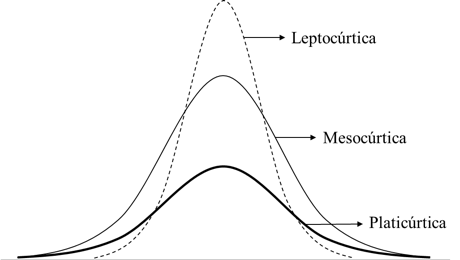
\includegraphics[scale=1]{Curticas.png}
\end{figure}


\end{itemize}


\newpage



\section{Trasformaciones de una variable aleatoria}

En muchas ocasiones estamos interesados en realizar operaciones de los datos procedentes de los experimentos aleatorios, bien porque es mas conveniente para su manipulación o porque es necesario para acceder a una nueva variable de interés. En general distinguimos dos tipos de trasformaciones: las lineales y las no lineales.  \\

\paragraph{Trasformaciones lineales.} 

Consideremos una muestra $\{ x_i \_{i=1}^N$ de realizaciones de la variable estadística $X$ con los posibles valores $\{ x_1, \ldots, x_k \}$ y media aritmética $\bar{x}$. Ahora si trasformamos esta variable a una nueva variable $Y = a + bX$ tenemos los valores posibles $\{ a +bx_1, \ldots, a + bx_k \}$. Analicemos ahora las principales medidas características de la nueva variable. La variable:

\begin{eqnarray}
\bar{y} & = & \sum_{i=1}^k f_i y_i =  \sum_{i=1}^k f_i (a + b x_i) \nonumber\\ 
        & = & a + b  \sum_{i=1}^k f_i x_i  = a + b \bar{x}
\end{eqnarray}


Como vemos la media aritmética se transforma de la misma manera que la variable. Por otra parte, la varianza de la nueva aleatoria será:

\begin{eqnarray}
s_y^2 & = & \sum_{i=1}^k f_i (y_i - \bar{y})^2 \nonumber\\
      & = & \sum_{i=1}^k f_i (a + bx_i -a -b\bar{x})^2 \nonumber\\
      & = & b^2 \sum_{i=1}^k f_i (x_i - \bar{x})^2 = b^2 s^2
\end{eqnarray}


\paragraph{Trasformaciones no lineales.}

En muchas veces usamos trasformaciones no lineales, por ejemplo:

$$ Y = X^P , \ Y = ln (X), \ Y = e^X \ldots $$

Las trasformaciones no lineales, suelen variar la forma de las distribuciones originales de frecuencias, lo que nos obliga a ser cuidadosos en el análisis de las implicaciones de la transformación en las diferentes medidas características. Veamos los efectos de este tipo de transformaciones en algunas medidas características.

\section{Distribuciones de frecuencia multivariable}

Al estudiar varias variables aleatorias obtenidas simultáneamente en un experimento podemos comprobar y hallar relaciones entre estas variables, usando distribuciones de frecuencia multivariante. \\

Si consideramos dos variables X e Y con valores \{$x_1$,...,$x_k$\} y \{$y_1$,...$y_l$\} tenemos que la frecuencia del par ($x_i, y_j$) será $f_{ij}$. \\

Llamamos \textbf{distribución de frecuencias marginal} para una variable X dentro de una distribución multivariante a la frecuencia asociada a los valores de X, sin importar los demás. Es decir es la frecuencia de que salga un $x_i$ determinado respecto a N sin importar si el par es $y_4$ o $y_7$. Es decir, si hablamos de frecuencias relativas:  

$$ f_{x_i} = \sum_j f_{ij} $$

\subsubsection{Independencia estadística y distribuciones de frecuencia condicionadas}


Cuando hablamos de frecuencia de $x$ condicionada a $y_j$ nos referimos a las diferentes probabilidades de que salga un $x_i$ \textit{sabiendo} que ha salido $y_j$. Es decir es la probabilidad de que salgan los diferentes $x_i$ sabiendo que la otra variable es una $y_j$ previamente definida. Entonces si $n_{y_j}$ es la frecuencia marginal de $y_j$ tenemos que las diferentes frecuencias de de $x_i$ condicionadas a $y_j$ son:

\begin{equation}
f(x_i | y_j) = \dfrac{f_{ij}}{n_{y_j}}
\end{equation}

Hablamos de \textbf{independencia estadística} entre x e y cuando las distintas distribuciones de $x_i$ condicionadas a cualquier $y_j $ son exactamente iguales que las distribuciones marginales de $x_i$. Entonces 

$$ f(x_i | y_j) = n_{x_i} = f_{x_i} $$

Es decir cuando la frecuencia de un $x_i$ no depende del $y_j$ que haya salido es cuando hablamos de \textit{independencia estadística}. 

\subsubsection{Medidas características muestrales multivariables}

Al igual que con las medidas normales aquí tenemos \textbf{momentos de la distribución}. LLamamos momento de ordenes r y s respecto al punto (c,d) como:

\begin{equation}
m_{r,s} (c,d)  = \sum_i \sum_j f_ {ij} (x_i-c)^r(y_j-d)^s
\end{equation}

Cuando hablamos momento respecto al origen hablamos momento respecto a (c,d)=(0,0) y momento central a (c,d)=($\bar{x}, \bar{y}$)

Para definir media de una de las variables estadísticas hablamos de:

\begin{equation}
\bar{x} = m_{1,0}(0,d) = \sum_i \sum_j f_{ij} (x_i-0)^1(y_j-d)^0
\end{equation}

Y la varianza como:

\begin{equation}
s_x^2=m_{2,0} (\bar{x},d) = \sum_i \sum_j f_{ij} (x_i-\bar{x})^2(y_j-d)^0 
\end{equation}

La \textbf{covarianza} es el momento central de primer orden en las dos variables estadísitcas (donde $\overline{xy}=\Sigma \Sigma f_{i,j} x_i y_j$):

\begin{equation}
\cov(x,y) = m_{1,1} (\bar{x}, \bar{y}) = \overline{xy} - \bar{x}\bar{y}
\end{equation}

Veamos ahora los cálculos para llegar a dicho resultado:
$$  \cov(x,y) = m_{1,1} (\bar{x}, \bar{y}) = \sum_i \sum_j f_{ij}(x-\bar{x})(y-\bar{y}) =  $$  $$ = \sum_i \sum_ j f_{ij} x_i y_j - \sum_i \sum_ j f_{ij} x_i \bar{y} - \sum_i \sum_ j f_{ij} y_j \bar{x} + \sum_i \sum_ j f_{ij} \bar{x} \bar{y}  = \overline{x y } - \bar{x}\bar{y} - \bar{x}\bar{y} + \bar{x}\bar{y}  $$


La covarianza tiene la característica que si x e y son independientes tiene valor de 0. Además informa sobre la correlación entre las variables estadísticas: si la covarianza es positiva hay una correlación positiva (como y=x) y si es negativa hay una correlación 
negativa (como y=-x). Véase mejor en la siguiente figura:  

\begin{figure}[h!] \centering
\includegraphics[scale=0.8]{covarianza.png}
\end{figure}

 \begin{figure}[h!] \centering
\includegraphics[scale=0.8]{covarianza1.png}
\end{figure}

Llamamos \textbf{coeficiente de correlación lineal entre variables estadísticas (X,Y)} como:
\begin{equation}
r_{x,y} = \dfrac{cov(x,y)}{s_x + s_y}
\end{equation}

Lo bueno de este coeficiente es que es adimensional ante cambios de escala (trasformaciones lineales), y su dominio está a cotado entre -1 y 1 siempre.  \newpage

\begin{figure}[h] \centering
\includegraphics[scale=0.7]{Correlación-lineal.png}
\end{figure}



\newpage

\chapter{Teoría de probabilidades}

\section{Fundamentos de probabilidad}
Llamamos \textbf{experimento aleatorio} a aquel que repetido sucesivas veces en condiciones idénticas produce diferentes resultados de manera no previsible. Un experimento determinista es aquel que repetido  veces en condiciones idénticas siempre produce el mismo resultado. Para ello introduciremos los siguientes conceptos básicos: 

\begin{itemize}

\item \textbf{Suceso elemental:} cada uno de los posibles resultados del experimento.

\item \textbf{Espacio muestral $\Omega$:} el conjunto de todos los resultados posibles. Un espacio muestral puede ser:

	\begin{itemize}
	
	\item \textbf{Discreto:} si cada uno de los sucesos se puede 				corresponder a un subconjunto de los números naturales
	
	\item \textbf{Continuo:} si cada uno de los sucesos se puede 				corresponder a uno o mas intervalos de la recta real
	
	\end{itemize}

\item \textbf{Suceso:} cualquier subconjunto del espacio muestral (por ejemplo que al tirar un dado sea par).

\item $\mathcal{A}$: es el conjunto de todos los sucesos que es posible definir asociados a un cierto experimento aleatorio.

\end{itemize}

Supondremos que el lector ya estará familiarizado con los conceptos de unión, intersección, conjunto vacío... así como distinguir la incompatibilidad, diferencia de varios sucesos. \\

Considérerse los sucesos A y B. Las \textbf{leyes de Morgan}, que son bastante intuitivas, nos dicen que:

\begin{itemize}

\item $ \overline{A \cup B} = \bar{A} \cap \bar{B}$:

\begin{figure}[h!] \centering
\includegraphics[scale=0.6]{primera-ley-morgan.png}
\end{figure}

\item $ \overline{A \cap B} = \bar{A} \cup \bar{B} $:


\begin{figure}[h!] \centering
\includegraphics[scale=0.7]{segunda-ley-morgan.png}
\end{figure}


\end{itemize}

Se define como \textbf{probabilidad de un suceso} (definición de probabilidad) como:

\begin{equation}
p(A) = \dfrac{\mathrm{casos \ favorables}}{\mathrm{casos \ posibles}} = \dfrac{n}{N}
\end{equation}

Cuando hablamos de probabilidad hay muchas cosas que, al igual que antes, daremos por conocidas, como que la probabilidad de la muestra es 1, la probabilidad del conjunto vacío es nula, que la probabilidad del complementario de A viene dada por 1 menos la probabilidad de A... Consecuentemente pasaremos a ver las probabilidades condicionadas, ya que tienen mucho mas interés. \\

Nosotros conocemos la probabilidad condicionada del suceso A respecto B como la probabilidad de que ocurra A sabiendo que ha ocurrido el proceso B:

\begin{equation}
p(A \vert B) = \dfrac{p(A \cap B)}{p(B)}
\end{equation}

Por consecuencia siempre que p(B) $>$ 0 podremos escribir que:

$$ p(A \vert B) p(B) = p(A \cap B) $$ \\

Decimos que dos procesos son \textbf{estadísticamente independientes} cuando: 
$$ p(A|B)=p(A) \Longleftrightarrow p(A \cap B)=p(A) \ p(B) \Longleftrightarrow p(B|A)=p(B) $$ 

Cuando los sucesos A y B son independientes los siguientes pares de sucesos también lo son: 

$$ A, \ \bar{B}; \quad \bar{A}, \ B; \quad \bar{A}, \bar{B} $$ \\

Llamamos a un conjunto de sucesos $ \{ A_1, A_2, ..., A_n | A_i \in \mathcal{A} \} $ es un \textbf{conjunto exhaustivo} si su unión cubre el espacio muestral: 

$$ U_{i=1}^n \ A_i=\Omega$$ \\
 
El mismo conjunto de sucesos se le llama \textbf{conjunto completo} si ademas los sucesos entre sí tienen intersecciones vacías. 
$$ A_i \cap A_j = \emptyset; \ p(A_i \cap A_j) = 0 \ \forall i \neq j $$ 

\Teorema{\textbf{Teorema de Bayes:} dado un suceso B el Teorema de Bayes nos indica que:
$$ p(A_i \vert B) = \dfrac{p(B \vert A_i) p(A_i)}{p(B)} = \dfrac{p(B \vert A_i) p(A_i)}{\Sigma_k p(B \vert A_k) p(A_k)}  $$}




\subsection{Función de probabilidad, densidad de probabilidad y distribución de probabilidad}

La función de \textbf{densidad de probabilidad se define como}:

$$ \lim_{\Delta\rightarrow 0} \frac{p(x_0 -\Delta \leq x \leq x_0 + \Delta)}{\Delta} = f(x_0) $$

Para esto la función de probabilidad p(x) tiene que ser suave. Además tiene las siguientes propiedades: 

\begin{itemize}

\item $f(x) \geq 0 \forall x \in  \R$ 

\item $ \int_{-\infty}^{\infty} f(x) \D x = 1 $

\item $ \int_{a}^{b} f(x) \D x = p(a \neq x \neq b) $ \\

\end{itemize}


La \textbf{función de distribución de probabilidad F(x)} se define como:

$$ F(x_0)  = p (x \leq x_0) = \int_{-\infty}^{x_0} f(x) \D x $$
Por lo tanto se cumplen las siguientes propiedades: 

\begin{itemize}

\item  $F(-\infty) = \lim_{x\rightarrow-\infty} F(x) = 0$

\item  $F(\infty) = \lim_{x\rightarrow\infty} F(x) = 1$ 

\item $\dfrac{\D F(x)}{\D x} = f(x)$

\end{itemize}

\subsection{Normalización de una distribución continua:}

Supongamos que tenemos una función de distribución de probabilidad definida como:

\begin{displaymath}
y = \left\{ \begin{array}{ll}
kx^2 & \textrm{si $0 \leq x \leq 2$}\\
0 & \textrm{en otro caos}\\
\end{array} \right.
\end{displaymath}


Entonces como la distribución de probabilidad tiene que cumplir que $\int_{-\infty}^{\infty} f(x) \D x = 1$ entonces:

$$ 1 = \int_0^2 k x^2 \D x = k \dfrac{8}{3} \Longrightarrow k = \frac{3}{8} $$

De esta forma tendríamos normalizada la función. 


\subsection{Esperanza:}

Dada una variable aleatoria definimos la esperanza o valor esperado de la variable como:

\begin{displaymath}
\E \{ X \} = \left\{ \begin{array}{ll}
\Sigma_i p(x_i) x_i & \textrm{si variable discreta}\\
 & \\
\int_{-\infty}^{\infty} f(x) x \D x & \textrm{si variable continua}
\end{array} \right.
\end{displaymath}

La esperanza de una variable aleatoria es su valor esperado, pero ¿Por qué? Cuando nosotros queremos calcular la media de cualquier cosa lo que hacemos es multiplicar la probabilidad de un que ocurra un suceso elemental por el propio suceso, eso en todos los sucesos posibles, sumarlos y dividirlos entre la cantidad de sucesos. En un caso integral lo que hacemos al poner x es poner estos sucesos elementales por su probabilidad (f(x)) en todo su espacio muestral (que es el que tenemos que recorrer). Por eso el valor esperado de una variable es igual a la esperanza del suceso. Podemos poner en vez de x H(x), siendo este un cambio de variable cualquiera y=H(x). Es el caso general. \\

En general solemos decir que la esperanza actúa como un operador lineal sobre la variable aleatoria, ya que:

$$ \E \{ \alpha H(X) + \beta G(X) \} = \alpha \E \lbrace H(X) \rbrace + \beta \E \lbrace G(X) \rbrace $$

\subsection{Medidas de centralización:}
Como ya dijimos la esperanza de la variable aleatoria X es igual al valor esperado (como la media). En general se escribe como:

\begin{equation}
\mu = \E \lbrace X \rbrace
\end{equation}

La \textbf{mediana Me} es el valor tal que F(Me)=0.5. La \textbf{moda Md} es el valor mas probable. Por consiguiente: 

$$ \left.  \dfrac{\D f}{\D x} \right|_{Md}  = 0$$ 

Por ser máximo. 

\subsection{Medidas de dispersión:}
La \textbf{varianza $\sigma^2$} de una variable aleatoria X se define como:

\begin{equation}
\sigma^2 = \E \corchetes{(X-\E \corchetes{X})^2} = \E  \corchetes {(X - \mu)^2}
\end{equation}

Y la  \textbf{desviación típica $\sigma$} es la raíz cuadrada de la varianza. La desviación típica cualitativamente nos trata de dar una medida de la dispersión de los datos. 

 
 

Las funciones de probabilidad pueden normalizarse (para que cuadren con las frecuencias relativas) y de esta forma su integral evaluada entre ($-\infty, \infty$). \\
  

\subsection{Tipificación de la variable aleatoria: \label{Subsec:2-tipificacion}}

Lo que hacemos al tipificar una variable aleatoria es mover la media al punto 0, de tal forma que no se cambia la forma,  ni la desviación típica; y luego crear una nueva variable donde "normalizamos" la varianza (de tal forma que $\sigma^2 = 1$. Para esto construimos una nueva variable tal que:

\begin{equation}
Y = \dfrac{X-\mu_x}{\sigma_x}
\end{equation}

$$ \E \corchetes{Y} =  \E \left\lbrace \dfrac{X - \mu}{\sigma} \right\rbrace  = \frac{1}{\sigma} \E \corchetes{X-\mu} =  \frac{1}{\sigma} \E \corchetes{X}  = 0  $$

$$ \sigma^2 (Y) = \EE{[Y^2- \EE{Y]}^2} = \EE{Y^2}  = \EEE{ \left[ \dfrac{X - \mu}{\sigma} \right] ^2} = \dfrac{1}{\sigma^2} \EE{(X- \mu)^2} = 1   $$

Dada cualquier variable aleatoria podemos tipificarla (haciendo ese cambio de variable). De esta forma podremos transformar cualquier variable aleatoria para poder así comparar variables aleatorias con diferente media y varianza, pudiendo caracterizar la dispersión, asimetría...

\subsection{Momentos de la distribución de probabilidad}

Definimos momento de orden j de una distribución de probabilidad de la misma manera que en estadística:
\begin{equation}
M_j (c) =  \E \{(x-c)^j\} = \int_{-\infty}^{+\infty} f(x)(x-c)^j
\end{equation}

De esta modo tenemos la media (momento respecto el origen de orden uno), la varianza (momento central de orden dos)...\\

\subsection{Función generatriz de momentos}

Muchas veces es mas fácil analizar las propiedades de una función de distribución de probabilidad usando les técnicas del análisis matemático mediante la \textbf{función generatriz de momentos}:

\begin{equation}
M_{x-c} (t) = \E \{ e^{[t(x-c)]} \} = \integral f(x) e^{t(x-c)} \D  x
\end{equation}

Entonces $M_{x-c}$ sea analítica (continua y diferenciable) en un intervalo:  

\begin{equation}
\dfrac{\D }{\D t} M_{x-c} (t) = \int_{-\infty}^{+\infty} f(x) (x-c) e^{[t(x_i-c)]} \D x
\end{equation}

Haciendo el límite cuando t tiende a cero tenemos que la primera derivada de la función generatriz de momentos es igual al momento de orden 1 respecto c.

\begin{equation}
\lim_{t \ \rightarrow \ 0} \dfrac{\D }{\D t} M_{x-c} (t) = \integral f(x) (x-c) \D x =  M_1(c)
\end{equation}

Si nos damos cuenta tenemos que: 

\begin{equation}
\lim_{t \ \rightarrow \ 0} (\dfrac{\D^j M_{x-c} (t)}{\D t^j}) = \integral f(x) (x-c)^j =M_j (c)
\end{equation}

Esto nos sirve para calcular momentos bastante altos de manera muy sencilla, incluso varianzas, curtuosis, asimetrías (fischer), medias... o el momento que queramos. Ahora veremos el ejemplo para la función de probabilidad exponencial:

\begin{displaymath}
f(x) = \left\lbrace 
\begin{array}{ll}
0 & x \in (-\infty,0) \\
\beta e^{-\beta x} & x \in[0,\infty)
\end{array} \right.
\end{displaymath}

Entonces tenemos que (c=0):

$$ M_x(t) = \integral f(x)  e^{t(x-c)} \D x = \int_0^{\infty} \beta e^{(t-\beta)x} \D x = \dfrac{\beta}{\beta - t} $$

Entonces si derivamos:

$$ \mu = M_1(x) = \lim_{t \rightarrow 0} \dfrac{\D M_x(t)}{\D t} = \lim_{t \rightarrow 0} \dfrac{\beta}{(\beta-t)^2} = \dfrac{1}{\beta} $$

$$ \sigma^2 = \EE {x^2} - \mu^2 = \lim_{t \rightarrow 0} \dfrac{\D^2 M_x(t)}{\D t^2} - \mu^2 = \lim_{t \rightarrow 0} \dfrac{2 \beta}{(\beta - t)^3} - \dfrac{1}{\beta^2} = \dfrac{1}{\beta^2}   $$

Entonces podremos calcular todos los momentos de distribución: 

$$ \dfrac{\D^r M_x(t)}{\D t^r} = \dfrac{r! \beta}{(\beta - t)^{r+1}} \Longrightarrow  M_0(x) = \dfrac{r!}{\beta^r} $$

\begin{center}
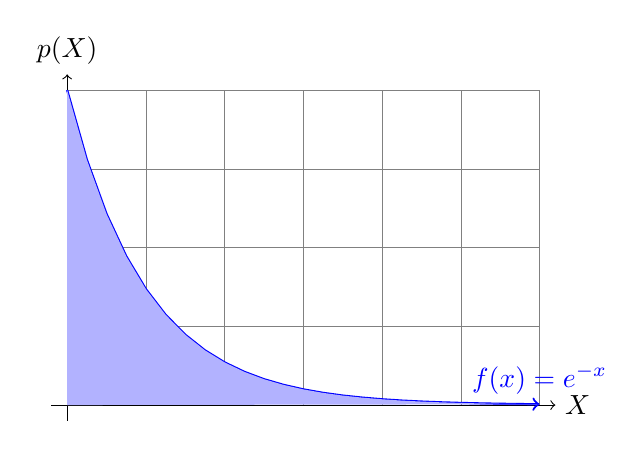
\begin{tikzpicture}
\draw[very thin,color=gray] (0,0) grid (6,4);
\draw[->] (-0.2,0) -- (6.2,0) node[right] {$X$};
\draw[->] (0,-0.2) -- (0,4.2) node[above] {$p(X)$};
\draw[blue,thick,->] plot[domain=0:6] (\x,{4*exp(-\x)}) 
	node[above] {$f(x) = e^{-x}$};

\fill[blue!30] (0,0)  -- plot[domain=0:6](\x, {4*exp(-\x)}) -- (0,0) -- cycle;
\end{tikzpicture}
\end{center}
\subsection{Transformación de la variable aleatoria:}

En el caso de una variable aleatoria continua (para variables aleatorias discretas se redefine de la misma manera) X podemos redefinirla mediante una aplicación g(x) tal que:

$$ y = g(x) $$

Siendo $f_X(x)$ y $f_Y(y)$ las funciones de densidad, tenemos que en un intervalo muy pequeño [a,b] de x la probabilidad de que ocurra esos mismos valores en y ([g(a),g(b)]) es exactamente la misma. Entonces:

$$ | f_Y(y) \D y |  = | f_X (x) \D x | $$

Es por el simple hecho de que si sale z veces los valores de X entre [a,b] tienen que salir z veces los valores de Y entre [g(a),g(b)]. Por lo tanto tenemos que:

\begin{equation}
f_Y(y)= \dfrac{f_X (x)}{|\frac{\D y}{\D x}|}
\end{equation}

Muchos nos podríamos preguntar para que sirve está trasformación, para que querríamos trasformar una variable aleatoria y crear una nueva función de densidad de probabilidad. Pues uno de sus mayores usos son los simuladores en los ordenadores. En la mayoría de ordenadores encontramos generadores aleatorios de distribución pero de distribución de probabilidad uniforme, sin embargo, si queremos simular la interacción radiación materia, la mayoría de los procesos  tiene una probabilidad de interacción exponencial. Entonces esta trasformación nos permitiría simular en el ordenador estas interacciones:

\begin{displaymath}
\left\lbrace \begin{array}{ll}
f_X(x) =1  & 0 \leq x \leq 1\\
f_Y (y) = \beta e^{-\beta x} & 0 \leq 0 < \infty
\end{array} \right. 
\end{displaymath}

$$ \left| \dfrac{\D y}{\D x} \right| = \dfrac{f_X(x)}{f_Y(y)} = \dfrac{1}{\beta e^{-\beta y}} \Longrightarrow (1-e^{-\beta y})=x \Longrightarrow y = \frac{-1}{\beta} \log(1-x) $$

Y ese sería el cambio de variable que hay que hacer para hacer la simulación. También nos interesa estudiar como se trasforma la media y la varianza de las variables aleatorias en un cambio de variable (y=g(x)). Podemos aproximar g(x) por la serie de taylor centrada en $\mu_x$:

$$g(x) = g(\mu_x) + \left. \dfrac{\D g}{\D x} \right|_{\mu_x} (x-\mu-x) + \dfrac{1}{2}  \left. \dfrac{\D^2 g}{\D x^2} \right|_{\mu_x} (x-\mu-x)^2 \ldots $$

Entonces:

$$ \EE{y} = \EE{g(x)} = g(\mu_x) + \left. \dfrac{\D g}{\D x} \right|_{\mu_x} \underbrace{\EE{(x-\mu_x)}}_{0} + \left. \dfrac{\D^2 g}{\D x^2} \right|_{\mu_x} \underbrace{\EE{(x-\mu_x)^2}}_{\sigma^2(x)} + \ldots $$

Entonces si podemos despreciar los términos de orden superior (a partir de dos) podemos despreciarlos y por lo tanto:

$$ \EE{Y} \approx g(\mu_x) $$ 

Podemos aplicar lo mismo para que:

$$ \sigma^2_Y \approx \left. \dfrac{\D g}{\D x} \right|_{\mu_x} \sigma^2_X $$

La demostración es análoga a la demostración de \ref{Ec:1.propagación-incertidumbres-trasformación-no-lineal}

\subsection{Distribución binomial:}
Para entender la distribución binomial primero debemos entender que es un \textbf{suceso de Bernouilli}: supongamos un suceso aleatorio con dos posibles resultados que asignaremos 0 y 1. Sea la probabilidad de 1 p (p(1)=p), y la probabilidad de 0 entonces será 1-p (p(0)=1-p=q). Para esta variable aleatoria tenemos que.

$$ \mu = \EE{x} = \sum_i p_i x_i = p + 0 = p $$

$$ \sigma^2 = \EE{(x-\mu)^2} = \sum_i p_i(x-i-p)^2 = p(1-p)^2 - q(0-p)^2 = pq(q+p)=pq $$

Ahora imaginemos que tenemos n sucesos de bernouilli estadísticamente independientes, como si tiráramos n veces una moneda. ¿Cuál es la probabilidad de que aparecieran, por ejemplo, x caras? Si p es la probabilidad de sacar una cara pues dependerá de los caminos posibles hasta llegar allí y la probabilidad de que ocurra uno de esos caminos. Ahora bien, ¿Cuál es la cantidad de caminos posibles? Si nos fijamos en este caso y vamos realizando el típico esquema:

\begin{figure}[h!] \centering
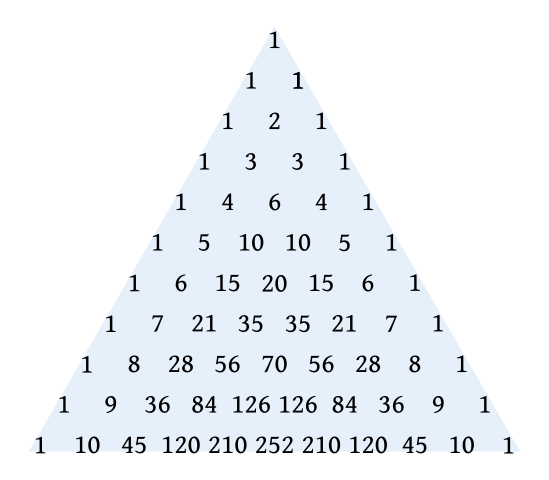
\includegraphics[scale=0.3]{triangulo-pascal.png}
\end{figure}

Tenemos que es el triángulo de pascal. Entonces la cantidad de caminos viene dada por la fórmula de la combinatoria: 

\begin{equation}
\binom{n}{r}= \dfrac{n!}{r!(n-r!)}
\end{equation}

Siendo n el número de tiradas y r el numero de veces que quieres que salga tu suceso. Y ahora: ¿Cuál es la probabilidad de que ocurra un camino? Pues está claro: la probabilidad de que ocurra el suceso que queremos r veces por la probabilidad de que no ocurra n-r veces. Entonces ya tendríamos formulado la probabilidad de que ocurra un proceso x veces, que sería:

\begin{equation}
p(x) = \binom{n}{x} p^x q^{n-x} = \dfrac{n!}{x! (n-x)!} p^x q^{n-x}
\end{equation}


Entonces el valor esperado y la varianza:

\begin{equation}
\EE{X} = \sum_{x=0}^n x p(x) = \sum_{x=0}^n x \binom{n}{x} p^x q^{n-x} =  \sum_{x=1}^n x \binom{n}{x} p^x q^{n-x} = np 
\end{equation}

\begin{equation}
\sigma^2 = \sum_{x=0}^n x p(x) = npq
\end{equation}

\Nota{escribir demostración}

\subsection{Distribución de Pascal:}
Se trata de evaluar el número de veces que se produce el experimento aleatorio hasta que el suceso A con probabilidad p no ocurra. La probabilidad de que siempre salga cara (probabilidad de que salga cara p) hasta que sale una cruz en n tiradas será:

$$ p(x=n)=p^{n-1}q $$

Entonces el valor medio de está será:

\begin{equation}
\mu = \sum_{x=0}^{\infty} x p^{r-1} = \dfrac{1}{q}
\end{equation}

\begin{equation}
\sigma^2 = \dfrac{p}{q^2}
\end{equation}

\Nota{escribir demostración} \\

En muchos libros nos podemos encontrar la definición contraria, cambiando n por q. Es decir que la distribución de pascal es la probabilidad de que un suceso A no ocurra hasta la n, de tal forma que:

$$ p(x=n) = q^{n-1}p $$


\subsection{Distribución de Poisson:}


En la distribución de Poisson es el límite de la distribución binomial si suponemos que el número de elementos (n) es muy grande pero la probabilidad de que ocurra un suceso (p) en un intervalo de elementos pequeño es realmente despreciable. Por ejemplo si cogemos la cantidad de accidentes de coche que hay en una carretera durante dos minutos, lo mas probable es que no ocurra ningún accidente. Sin embargo si cogemos la probabilidad a lo largo de 1 mes es probable encontrar un resultado de tal manera que la probabilidad de que p haya ocurrido sea una constante ($\lambda$) que se repita todos los meses que lo hagamos, incluso  que si lo hagamos 10 años la probabilidad de accidentes sea la misma (no la cantidad). Entonces tenemos que para sucesos con n grande el valor esperado se mantiene constante:

\begin{equation}
\EE{x}=\lambda=np; \ p = \lambda/n
\end{equation}

Entonces tenemos que:

$$
p(x=r) = \binom{n}{r}(\dfrac{\lambda}{n})^r (1-\dfrac{\lambda}{n})^{n-r} 
$$

Del cual podemos tomar los límites n $\rightarrow \infty$ de tal manera que (siendo x el número de intentos):

\begin{equation}
p(x=r)= \dfrac{\lambda^r}{r!} e^{-\lambda}
\end{equation} 

\begin{equation}
\EE{x} = \lambda 
\end{equation}

\begin{equation}
\sigma^2 = \lambda
\end{equation}

\Nota{escribir demostraciones}

\subsection{Distribución Gaussiana:}

Una variable aleatoria continua se dice que tiene una distribución de probabilidad gaussiana cuando su densidad de probabilidad se puede escribir como:

\begin{equation}
f(x) = \dfrac{1}{\sqrt{2 \pi} \sigma} e^{-\frac{(x-\mu)^2}{2  \sigma^2}}; \quad \sigma>0, \ \ x \in (-\infty, \infty)
\end{equation}

\begin{center}
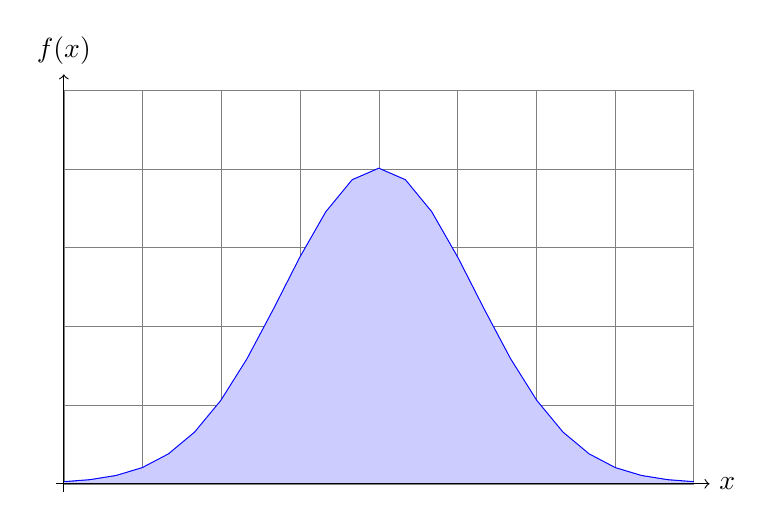
\begin{tikzpicture}[domain=0:8][scale=0.4]
    \draw[very thin,color=gray] (0.0,0.0) grid (8,5);
    \draw[blue,thick] plot[domain=0:8] (\x,{4*exp(-((\x -4)^2)/3)}) ;
	\fill[blue!20] (0,0)  -- plot[domain=0:8](\x, {4*exp(-((\x -4)^2)/3)}) -- (8,0) -- (0,0) -- cycle;
	
    \draw[->] (-0.1,0) -- (8.2,0) node[right] {$x$};
    \draw[->] (0,-0.1) -- (0,5.2) node[above] {$f(x)$};
\end{tikzpicture}
\end{center}

Y su función de distribución de probabilidad:

\begin{equation}
F(x) = \dfrac{1}{\sqrt{2 \pi} \sigma} \int_{-\infty}^{x} e^{ - \frac{(t-\mu)^2}{  2 \sigma^2}} \D t; \quad \sigma>0 x \in (-\infty, \infty)
\end{equation}
Entonces podríamos probar que:

\begin{equation}
\EE{x} = \mu 
\end{equation}

\begin{equation}
\sigma^2 = \sigma^2
\end{equation}

Normalmente escribimos la gaussiana de media $\mu$ y desviación típica $\sigma$:

$$ x \in N(\mu, \sigma) $$

Si calculamos la función generatriz de momentos para la \textbf{función normal estándar} (gaussiana $\mu=0$, $\sigma=1$) tenemos que: 

$$ M_X(t) = \EE{e^{tx}} = \integral  f(x) e^{ tx} \D x = \integral \frac{1}{\sqrt{2 \pi} \sigma} e^{tx - \frac{(x - \mu)^2}{2 \sigma^2}} \D x =  \integral \frac{1}{\sqrt{2 \pi}} e^{tx - \frac{x^2}{2}} \D x \Longrightarrow $$

$$ M_X (t) = \integral \frac{1}{\sqrt{2 \pi}} e^{-\frac{(t-x)^2}{2}} e^{\frac{t^2}{2}}D x  = e^{t^2 /2} (2\pi)^{-1/2} \underbrace{\int e^{-(t-x)^2 /2}}_{(2\pi)^{1/2}} \Longrightarrow$$

\begin{equation}
M_X(t) = e^{\frac{t^2}{2}}
\end{equation}

En general podemos convertir cualquier gaussiana a una normal estándar  gracias a la tipificación que vimos en \ref{Subsec:2-tipificacion}. Si calculamos la \textbf{curtuosis} de la distribución normal tenemos que ($\sigma = 1; \ \mu=0$; como la media es 0 podemos calcular la curtuosis directamente como la derivada cuarta de la función generatriz de momentos):

$$  g = \frac{M_4(\mu)}{\sigma^4} = \left. \frac{\D^4 e^{t^2/2}}{\D t^4} \right| _0 = \lim_{t \rightarrow 0} 3 e^{t^2/2} + 6t^2 e^{t^2/2} + t^4 e^{t^2/2} = 3 $$

\subsection{Distribuciones multivariables}

Un suceso muchas veces implica calcular determinadas magnitudes a la vez. En este caso a la variable aleatoria se le llama \textbf{variable aleatorias multidimensionales o vectoriales} . Por ejemplo, al medir la estatura el peso y la edad en la población española resulta una variable aleatoria tridimensional, además que las 3 estarán relacionadas mediante una correlación (la estudiaremos mas adelante con la covarianza). En este caso el valor de la variable aleatoria es un conjunto de n valores numéricos. \\

Entonces para las distribuciones multivariables definiremos una función de probabilidad  conjunta f(x,y). Llamamos distribuciones marginales para una de las componentes $x_i$ de la distribución a la probabilidad de que salgan os diferentes valores de $x_i$ ignorando las otras variables. Es decir consideramos la distribución univariante de dicha componente, su distribución en la población considerada aisladamente. De este modo sea la distribución bidimiensional f(x,y):

\begin{itemize}
\item $f(x)=\integral f(x,y) \D y$
\item $f(y)=\integral f(x,y) \D x $

\end{itemize}

Además, como en el Tema \ref{Sec:estadística} podemos hablar de independencia estadística y de probabilidades condicionadas. En el caso bidimensional (de ahora en adelante trataremos siempre el caso bidimensional, a menos que especifiquemos que no) tenemos que x e y son independientes estadísticamente si se cumple que:

$$ f(x|y)=f(x); \ f(y|x)=f(y) \ / \ f(x|y)=\dfrac{f(x \cap y)}{f(y)} $$

También tenemos el \textbf{teorema de bayes} para distribuciones multivariables, medias, varianza, momentos... Quizás lo mas relevante sería la \textbf{covarianza}, ya que nos da una medida de la correlación entre las variables. Por ejemplo si dos variables son estadísticamente independiente tenemos que la covarianza es 0. Sin embargo \underline{el recíproco no es cierto}. Definimos covarianza como:ç


\begin{equation}
\cov  (x,y) = \integral \integral (x-\mu_x)(y-\mu_y)f(x,y) \D x \ \D y
\end{equation}

\Nota{demostrar que si dos variables estadísticamente independientes su covarianza es 0}

\subsection{Sumando variables aleatorias y Teorema del límite central:}

Consideremos dos variables aleatorias X e Y, tal que construimos una nueva variable  Z = X + Y. Entonces la media y la varianza de Z vendrán dadas por:

\begin{equation}
\EE{z} = \EE{x} + \EE{y}
\end{equation}
\begin{equation}
\sigma_z^2 = \sigma_x^2 + \sigma_y^2 + 2 \cov(x,y)
\end{equation}

Y si X e Y son independientes estadísitcamente $\cov (x,y)=0$ y por lo tanto: 

$$ \sigma_z^2 = \sigma_x^2 + \sigma_y^2  $$

Entonces si consideramos que sumamos n variables aleatorias independientes  ($X_1, X_2, ..., X_N$) con la misma distribución de probabilidad de tal manera que la media de $X_i$ es $\mu$ y la varianza $\sigma^2$. Entonces si definimos una variable aleatoria $\bar{X}$ tal que: 

$$\bar{X} = \frac{1}{n}(X_1+X_2+X_3+...+X_N)$$

La media y varianza de $\bar{X}$ vendrá dada por:

$$ \EE{\bar{X}} = \mu; \  \sigma^2(\bar{X})=\dfrac{\sigma^2}{n} $$

Si tipificamos la variable aleatoria $\bar{X}$ tenemos que:

\begin{equation}
\bar{Y}=\dfrac{\bar{X}-\mu}{\frac{\sigma}{\sqrt{n}}}
\end{equation}

Tal que $\mu_Y=0$ y $\sigma_Y = 1$. Tenemos que si $n \rightarrow \infty$ la probabilidad de $\bar{Y}$ tiene una distribución de probabilidad igual que una normal estándar N(0,1). \\

\Nota{demostrar esto }
\newpage

\chapter{Métodos estadísticos}

En los métodos estadísticos estudiamos los métodos mediante los cuales podamos hacer afirmaciones o predicciones acerca del comportamiento de los elementos de una población a partir de la observación de subconjuntos de la población llamadas muestras. A este estudio también se le llama \textbf{inferencia estadística}, y en esta sección se introduciran los siguientes temas:

\begin{enumerate}
\item \textbf{Estimación puntual y por intervalos:} en esta parte estudiamos las técnicas de estimación de parámetros de distribuciones de probabilidad a partir de los obtenidos en las distribuciones de frecuencia experimentales o empíricas. El caso mas importante es aquel en el que consideramos una población en la que tenemos definida una función de distribución de probabilidad. La información ($\mu, \sigma...$) de las distribuciones serán desconocidas, y tendremos que calcularlas a partir de nuestros datos experimentales mediante una serie de procedimientos. En particular nos centraremos en el tratamiento detallado de la estimación puntual de la media y varianza, así como la construcción de intervalos de confianza para estos.

\item \textbf{Test de hipótesis estadísticas:} gracias a los test de hipótesis estadísticas podremos estimar el nivel de aceptabilidad estadística de una afirmación acerca del comportamiento de una población con la información conocida de una muestra.

\item \textbf{Método de máxima verosimilitud:} proporciona un procedimiento de evaluación de los parámetros que maximiza la probabilidad de obtención de los datos determinada a una distribución. De esta forma podremos maximizar los parámetros de un ajuste (lineal, exponencial...) para maximizar la verosimilitud de la muestra (una vez suponemos que la muestra sigue una determinada distribución de probabilidad).
\end{enumerate}


\subsection{Estimación puntual de parámetros}
Si consideramos una población de todas las posibles medidas de una magnitud de interés, siendo X la variable aleatoria y f(x) la función densidad de probabilidad, existen ciertos parámetros que describen esta distribución de probabilidad, tales como la media, la desviación típica, la curtuosis...  \\

Para resolver el problema primero debemos tener los datos que hemos obtenido. Considerando que tomamos $l$ muestras de tamaño $n$; y consideramos que cada una de las muestras corresponden a una variable n dimensional:

$$ \vec{x} \ ^i = (x_1^i, x_2^i, \ldots,  x_n^i) $$

Que siguen una distribución de probabilidad multivariante $g(\vec{x})$. Para poder garantizar que nuestro estudio se realiza en las mejores condiciones (y las mas senciallas de calcular) supondremos que:

\begin{itemize}
\item Todas las medidas son independientes entre sí: no hay correlación entre las medidas de una muestra.

\item Las distribuciones de cada medida son idénticas entre sí, e iguales a la distribución de probabilidad de la población:

$$ g_1 (x_1) = g_2 (x_2) = \cdots = g_n(x_n) = f(x)$$
\end{itemize}

En general estas condiciones se dan en muchas medidas físicas aunque no son absolutas: podemos desconocer la distribución de probabilidad, o que no describa el comportamiento de la población; incluso no saber si realmente las medidas son estadísticamente independientes. Aquellas muestras que cumplan estas condiciones se le llaman \textbf{muestras aleatorias simples}. \\

Llamamos \textbf{estadístico} a una función de las variables estadísticas. Un estadístico es una variable aleatoria por el simple hecho de que son funciones de variables aleatorias. Por lo tanto un estadístico sigue una función de probabilidad. Lo veremos mas adelante. \\

Un \textbf{estimador S} de un parámetro $\lambda$ cualquiera a un estadístico o función que nos permita estimar el parámetro que deseamos conocer:

$$ S = S(x_1, x_2, \ldots, x_n) $$

Para que un estimador este correctamente definido tiene que cumplir una serie de características, que son:

\begin{enumerate}
\item \textbf{Fidelidad:} se dice que un estimador lineal es fiel si para cualquier tamaño n de la muestra se cumple que:

\begin{equation}
\EE{S(x_1, x_2, \ldots, x_n)}= \lambda
\end{equation}

\item \textbf{Consistencia:} un estimador se dice consistente si aumenta en precisión con el tamaño de la muestra:

\begin{equation}
\lim_{n \rightarrow \infty}  \sigma(S) = 0
\end{equation}

\item \textbf{Eficiencia:} entre dos estimadores fieles y consistentes la eficiencia relativa será:

\begin{equation}
\eta = \dfrac{\EE{(S_1-\lambda)^2}}{\EE{(S_2-\lambda)^2}} = \dfrac{\sigma^2(S_1)}{\sigma^2(S_2)}
\end{equation}

Siempre es preferido aquel estimador con la varianza mas pequeña, y la eficiencia nos puede ayudar a escoger entre varios estimadores, en el caso de duda.

\end{enumerate}

\subsubsection{Estimación puntual de la media poblacional}

La media poblacional $\mu$ es fundamental en la estadística para la construcción de probabilidad de un fenómeno.  Si consideramos el caso de un muestreo aleatorio simple con una distribución de probabilidad $f(x)$ del que hemos tomado los datos $\corchetes{x_i}_{i=1}^n$. El mejor estimador de la media poblacional será la media muestral $\bar{x}$, que se define como:

\begin{equation}
\bar{x} = \dfrac{1}{n} \sum_{i=1}^n x_i
\end{equation}

Para realmente comprobar que es el mejor (más eficiente, fiel y consistente) estimador de la media poblacional deberíamos comprobar punto por punto los anteriores requisitos anteriormente seleccionados. Sin embargo esto escapa de la intención de estos apuntes, muy básicos. En el caso de querer saber mas recomendamos la lectura de la bibliografía. \\

Como hemos dicho un estadístico es una variable aleatoria (ya que procede de variables aleatorias). Entonces el propio estadístico también sigue una distribución aleatoria. Ahora bien, ¿Cuál es la distribución que afecta a nuestro estadístico media muestral? Si la distribución de población madre (la de nuestras variables aleatorias iniciales) $f(x)$ es normal entonces la suma de $n$ variables normales seguirá una distribución normal. Entonces $\bar{x}$ será una variable aleatoria de media $\mu$ y varianza $\sigma^2/n$, es decir $N\parentesis{\mu, \frac{\sigma}{\sqrt{n}}}$. Y si tipificamos y encontramos el cambio de variable: 

\begin{equation}
z = \dfrac{\bar{x}-\mu}{\sigma/\sqrt{n}}
\end{equation}

Tenemos que z seguirá una normal $N(0,1)$. Aun en el caso de que $f(x)$ no siga una densidad de probabilidad gaussiana, si tiene momentos finitos sabemos que sumando las suficientes variables aleatorias (es decir con una muestra lo suficientemente grande), la distribución de la media tenderá a una gaussiana. 

\subsubsection{Estimación puntual de la varianza poblacional}
Otro de los parámetros fundamentales de una distribución cualquiera es la anchura de la distribución, es decir, la varianza poblacional $\sigma^2$. Podríamos suponer que la varianza poblacional viene dado por el siguiente estimador:

$$ \grave{s}^2  = \dfrac{1}{n} \sum_{i=1}^n (x_i - \bar{x})^2 $$

Pero a la hora de valorar su fidelidad nos aparece que:

$$ \EE{\grave{s}^2} = \dfrac{n-1}{n} \sigma^2 $$

Por lo que este estimador no es fiel. Debido a la linealidad de la esperanza podríamos obtener que un estimador fiel sería:

$$ \dfrac{n}{n-1} \EE{\grave{s}^2} = \sigma^2 \Longrightarrow \E \underbrace{\Corchetes{\frac{n}{n-1} \ \grave{s}^2}}_{s^2} = \sigma^2 $$

Entonces el estimador lineal $s^2$ si sería fiel, y lo podríamos construir de la siguiente forma:

\begin{equation}
s^2 = \dfrac{1}{n-1} \sum_{i=1}^n (x_i - \bar{x})^2
\end{equation}

La aparición de un factor $n-1$ no es casualidad, ya que al introducir en la definición del estadístico un estadístico estamos imponiendo una ligadura entre los valores, ya que $\bar{x}$ y $\corchetes{x_i}_{i=0}^n$ no son linealmente independientes. Es decir $n-1$ son los grados de libertad del estimador $s^2$. Si $n=1$ (solo tenemos un dato) esta forma de estimar la varianza sería bastante errónea. \\


En muchos casos la distribución de la varianza tiene un comportamiento asimétrico. Su forma depende tanto de $f(x)$ como de $n$. De forma general se puede demostrar que el siguiente estimador lineal depende de una función llamada la chi cuadrada de person $\chi^2$ con $n-1$ grados de libertad:

\begin{equation}
\dfrac{(n-1)}{\sigma^2} s^2  =\sum_{i=1}^n \dfrac{(x_i-\bar{x})^2}{\sigma^2} = \chi^2_{n-1}
\end{equation}



La $\chi^2$ tiene propiedades muy interesantes como:

\begin{enumerate}
\item La distribución de probabilidad de suma de dos variables que se comporten como $\chi^2$ con $n_1$ y $n_2$ grados de libertad respectivamente es una variable que se comporta como una $\chi^2$ de $n_1+n_2$ grados de libertad. 
\item El valor esperado de una distribución $\chi^2$ es $n$.
\item La varianza de una distribución $\chi^2$ es $2n$. 
\end{enumerate}

Definiéndose la distribución de $\chi^2$ para n grados de libertad con $\lambda = \frac{n}{2}$ como:

\begin{equation}
f(\chi^2) = \dfrac{1}{\Gamma (\lambda) 2^{\lambda}} \parentesis{\chi^2}^{\lambda-1} e^{-\chi^2/2}
\end{equation}

\subsubsection{Distribuciones de $\bar{x}$ para poblaciones madre normales}


Como hemos mencionado si la variable aleatoria $X$ tiene una distribución normal entonces $\bar{x}$ tiene una distribución $N(\mu, \frac{\sigma}{\sqrt{n}})$. Si la función madre no tiene una distribución normal pero la muestra tiene un numero suficiente de datos ($n\geq 30$) podemos crear un cambio de variables tal que $z=\frac{x-\mu}{\sigma}$ de tal modo que la distribución se aproxime a una normal $N(0,1)$. Sin embargo, muchas veces (o mas bien casi nunca) conocemos el valor de la varianza poblacional, y tenemos que usar nuestro estimador de la varianza poblacional, la varianza muestral $s^2$.  En ese caso el cambio de variable será:

\begin{equation}
t = \dfrac{\bar{x}-\mu}{s/\sqrt{n}}
\end{equation}

Como podemos ver el cambio que se ha hecho es:

\begin{equation}
\sigma(\bar{x}) \simeq \dfrac{s}{\sqrt{n}} = \sqrt{\dfrac{\sum{(x_i-\bar{x})^2}}{n (n-1)}}
\end{equation}

Entonces podemos reescribir esto de tal forma que:

$$ t = \dfrac{\frac{\bar{x}-\mu}{\sigma \sqrt{n}}}{s/\sigma} = \dfrac{\frac{\bar{x}-\mu}{\sigma \sqrt{n}}}{\sqrt{\frac{\chi^2_{n-1}}{n-1}}} $$

Sea $z$ una variable normal distribuida según $N(0,1)$ y sea una variable $\chi^2_n$ distribuida según la chi cuadrado de Pearson con n grados de libertad tenemos que la variable

\begin{equation}
t_n = \dfrac{z}{\sqrt{\frac{\chi^2_n}{n}}}
\end{equation}

sigue una distribución $t$ de Student con $n$ grados de libertad cuya densidad de probabilidad es:

\begin{equation}
f(t) = \dfrac{\Gamma (\frac{1}{2}(n+1))}{\Gamma (\frac{1}{2}n) \sqrt{\pi} \sqrt{n}} \parentesis{1+\dfrac{t^2}{n}}^{-\frac{1}{2} (n+1)}
\end{equation}

De todo esto podemos deducir que la distribución de la media muestral $\bar{x}$ en el caso de no conocer la varianza poblacional $\sigma^2$ sigue una distribución $t$ de student con $n-1$ grados de libertad (tras hacer el cambio de variables...). Cuando $n$ es pequeña esta distribución de probabilidad es mas ancha que la normal, sin embargo si $n$ es lo suficientemente grande la $t$ de student tiende a una distribución gaussiana normal. 

\subsection{Intervalos de confianza}

Normalmente, cuando tratamos de estimar un parámetro no solo nos interesa obtener un valor puntual, si no el rango donde debería encontrarse el verdadero valor del parámetro, con un determinado nivel de probabilidad o confianza. Recordemos que los propios estimadores son, a fin de cuentas, variables estadísticas que tienen incertidumbre. Aunque los intervalos de confianza se pueden dar a cualquier estimador (incluso el de la incertidumbre), en estos apuntes solo analizaremos los intervalos de confianza de la media poblacional estimada a partir de la media muestral y los intervalos de confianza para la estimación de la varianza a partir de la muestra en poblaciones madre normales (solo este caso). 



\subsubsection{Intervalos de confianza para la media poblacional}

El objetivo ahora es obtener un rango, un intervalo en el cual con una probabilidad $1 - \alpha$ se encuentre la media poblacional $\mu$. Entonces la probabilidad de que $\mu$ este en el intervalo $(a,b)$ será:

$$ P(a < \mu < b) = 1 - \alpha $$   

A $1 - \alpha$ lo conocemos como el nivel de confianza y definirá el tamaño del intervalo. Para construir este intervalo de confianza nos apoyaremos en $\bar{x}$. Normalmente nos encontramos que nos dan un nivel de confianza en tanto por cierto, pero otras muchas nos dan la probabilidad de error. La probabilidad de error no es mas que el valor de $\alpha$, expresado también en tanto por ciento muchas veces. Estudiaremos ahora diferentes intervalos de confianza para la media poblacional, para poblaciones madre normales.  \\


\paragraph{A) Intervalo de confianza para la media $\mu$ de una población madre con $\sigma$ conocida \\ \\ }

Es obvio que si consideramos un intervalo $(a,b)$ donde $\mu$  se encuentre con una probabilidad $1- \alpha$, que la media se ecuentre por la izquierda ($x<a$) como por la derecha del  ($b<x$)del intervalo tendrá una probabilidad de $\alpha/2$.\\

Dado que estamos considerando una población madre de la muestra de datos normal, de $\sigma$ conocida. Entonces podemos crear una normal $N(0,1)$ a partir de la variable alatoria:

$$ z = \dfrac{\bar{x}-\mu}{\sigma / \sqrt{n}} $$

Esta nueva variable nos permitirá estimar la media poblacional. El intervalo que buscamos lo podremos obtener a partir de los percentiles de la distribución normal estándar que dejan a su izquierda y derecha un área igual a $\alpha/2$. El valor en el que justamente toda el área hasta ese momento ocupa dicha área lo llamaremos $-z{_\alpha/2}$. Para el caso de área superior $z{_\alpha/2}$. Entonces:

\begin{equation}
- z_{\alpha/2} \leq  \dfrac{\bar{x}-\mu}{\sigma / \sqrt{n}} \leq z_{\alpha/2}
\end{equation}

Lo cual implica que el intervalo de confianza será:

\begin{equation}
\bar{x} - \frac{\sigma}{\sqrt{n}} \ z_{\alpha/2} \leq \mu \leq  \bar{x} + \frac{\sigma}{\sqrt{n}} \ z_{\alpha/2}
\end{equation}

Ahora imaginemos que tenemos una población, y queremos obtener el tamaño de la muestra para que con una probabilidad $1-\alpha$ la diferencia entre la media muestral $\bar{x}$ y la media poblacional $\mu$ sea menor que $D$. Es decir, trataremos de obtener el tamaño de la muestra para el cual la media poblacional este a una distancia máxima D del valor verdadero con una probabilidad determinada. Entonces con estas consideraciones:

\begin{equation}
 -\frac{\sigma}{\sqrt{n}} \ z_{\alpha/2}  \leq \mu \leq   \frac{\sigma}{\sqrt{n}} \ z_{\alpha/2}
\end{equation}

Por lo que la diferencia máxima $D$:

\begin{equation}
D = z_{\alpha/2}  \dfrac{\sigma}{\sqrt{n}}
\end{equation}

Y si despejamos $n$:

\begin{equation}
n =  \dfrac{z^2_{\alpha/2} \sigma^2}{D^2}
\end{equation}

\paragraph{B) Intervalo de confianza para la media $\mu$ de una población madre con $\sigma$ desconocida \\ \\}


En este caso la diferencia es que en vez de obtener los percentiles y valores a partir de una normal $N(0,1)$ usando el cambio de variable z, usaremos la $t$ de student para evaluar el intervalo de confianza. Entonces si consideramos exactamente lo mismo para el parámetro $t$:

$$  t = \dfrac{\bar{x}-\sigma}{s/\sqrt{n}}$$

Que seguirá la distribución $t$ de student con $n-1$ grados de libertad. Entonces para este caso:

\begin{equation}
- t_{\alpha/2} \leq  \dfrac{\bar{x}-\mu}{s / \sqrt{n}} \leq t_{\alpha/2}
\end{equation}

Lo cual implica que el intervalo de confianza será:

\begin{equation}
\bar{x} - \frac{s}{\sqrt{n}} \ t_{\alpha/2} \leq \mu \leq  \bar{x} +  \frac{s}{\sqrt{n}} \ t_{\alpha/2}
\end{equation}

Recordemos que la $t$ de student cambia en función del número de datos a considerar. 

\subsubsection{Intervalos de confianza para la varianza $ \sigma^2 $ de una distribución normal}

Como hemos visto la variable aleatoria $(n-1)s^2/\sigma^2$ sigue una distribución $\chi^2$ de Pearson con n-1 grados de libertad. Ahora introduciremos un pequeño cambio, muy sutil respecto a lo anterior. Denotaremos como $\chi^2_{\alpha/2,n}$ el valor que deja a su derecha un área $\alpha/2$. Entonces:

\begin{equation} 
P\left[ \chi^2_{1 - \alpha/2,n-1} \leq \dfrac{(n-1)s^2}{\sigma^2} \leq \chi^2_{ \alpha/2,n-1} \right] = 1 - \alpha
\end{equation}

De lo que podemos deducir que:

\begin{equation}
P \left[ \dfrac{(n-1)s^2}{\chi^2_{\alpha/2,n-1}} \leq \sigma^2 \leq \dfrac{(n-1)s^2}{\chi^2_{1 - \alpha/2,n-1}} \right] = 1 - \alpha
\end{equation}

Muchas veces en realidad no nos importa que la sigma se encuentre por debajo de el intervalo. De hecho, hasta nos conviene: cuanto mas se acerque a cero mejor, ya que significa que el experimento está mejor realizado. Entonces en ese caso podemos reescribir todo esto, teniendo en cuenta que ahora $\chi^2_{1-\alpha,n}$ es aquel valor que deja a la derecha a la variable aleatoria $\chi^2_{\alpha/2,n}$ con un nivel de confianza $\alpha$. Entonces como antes: 

\begin{equation} 
P\left[ \chi^2_{1 - \alpha,n-1} \leq \dfrac{(n-1)s^2}{\sigma^2} \right] = 1 - \alpha
\end{equation}

De lo que podemos deducir que:

\begin{equation}
P \left[ \sigma^2 \leq \dfrac{(n-1)s^2}{\chi^2_{1 - \alpha ,n-1}} \right] = 1 - \alpha
\end{equation}

\subsection{Test de hipótesis estadísticas}

Una hipótesis estadística es una afirmación que se realiza sobre una o mas características de la población. Una hipótesis de este tipo, puede ser, por ejemplo, la afirmación de que la fuerza que se ejerce sobre un muelle es proporcional al estiramiento del mismo con una constante $k$. Hipótesis de este tipo deben ser verificadas o contrastadas mediante la observación empírica o experimental de un fenómeno. Una hipótesis estadística estaría completamente contrastada si pudiéramos verificarlo con todos los elementos de la población, pero dado que la población tiene infinitos elementos (o no es accesible conseguirlos todos) en general la verificación estadística de una hipótesis se realiza mediante muestras de la población. \\

Consideramos dos tipos de hipótesis. La hipótesis simple y la hipótesis compuesta se diferencial principalmente en que la hipótesis simple establece un valor concreto para el parámetro de estudio (o varios) y la compuesta afirma un intervalo o recorrido para ellos. \\

El test de hipótesis alternativas se presenta mediante la contraposición de dos hipótesis, una que afirma lo que queremos que afirme (por ejemplo que el valor de la constante es $k$) y otra que considera todos los demás casos. Se llaman, respectivamente, hipótesis nula $H_0$ e hipótesis alternativa $H_a$:

\begin{gather}
\begin{array}{lll}
H_0 \ ; \ \mu = \mu_0 & \rightarrow & \text{hipótesis nula} \\
H_a \ ; \ \mu \neq \mu_0 & \rightarrow & \text{hipótesis alternativa} 
\end{array}
\end{gather}

El proceso de test de una hipótesis estadística sigue los siguientes pasos:

\begin{enumerate}
\item Definición de una hipótesis nula $H_0$ y una hipótesis alternativa $H_a$
\item Definición de una medida de discrepancia entre los datos muestrales y la hipótesis $H_0$. Para ello un función de los datos de la muestra.
\item  Definición de la región de aceptación de $H_0$, constituida por el conjunto de valores que consideramos aceptable si $H_0$ es cierta. Para ello debemos fijar un nivel de significación $\alpha$ que es la probabilidad de rechazar $H_0$ siendo correcta. En general es la probabilidad de fallar en la decisión de descartar o aceptar la hipótesis. La probabilidad de aceptar $H_0$ siendo falsa se denota por $\beta$. A estos parámetros se les suele llamar error de tipo I y tipo II respectivamente.
\item Cálculo de la función de decisión llamado estadístico de contraste para aceptar o rechazar $H_0$.
\end{enumerate}

Ahora analizaremos diferentes test de hipótesis estadísticas.


\subsubsection{Test de la media de una población normal}

Consideremos una población gaussiana de media $\mu$. Entonces:

\begin{gather}
\begin{array}{ll}
H_0 \ : & \mu = \mu_0 \\
H_a \ : & \mu \neq \mu_0
\end{array}
\end{gather}

Escogemos como estadístico de contraste: 

$$ t = \dfrac{\bar{x}-\mu_0}{s/\sqrt{n}} $$

Evidentemente mide la distancia (normalizada, ya que esta divido entre la incertidumbre) entre los datos muestrales y la hipótesis estadística. Este estadístico sigue una $t$ de Student con $n-1$ grados de libertad. La región crítica $c$ es el valor de $t$ para el cual rechazamos la hipótesis a un nivel de confianza $1-\alpha$. 

\begin{equation}
c = \{ t: |t| > t_{\alpha/2; n-1} \}
\end{equation}

Y la región de aceptación:

\begin{equation}
\Delta = \{ t: |t| \leq t_{\alpha/2; n-1} \}
\end{equation}

Aceptando la hipótesis si:

\begin{equation}
 \dfrac{|\bar{x}-\mu_0|}{s/\sqrt{n}} \leq t_{\alpha/2; n-1}
\end{equation}

Y rechazándola si:

\begin{equation}
 \dfrac{|\bar{x}-\mu_0|}{s/\sqrt{n}} > t_{\alpha/2; n-1}
\end{equation}

Entonces podremos aceptar la hipótesis siempre que el estadístico se encuentre en la región $\Delta$, o rechazarlo si está en la región $c$. Este contraste es de tipo bilateral, ya que lo rechazamos o aceptamos la hipótesis si el estadístico se encuentra por debajo o por encima de unos valores. Si solo quisiéramos rechazar datos en que el estadístico estuviera por encima o por debajo de unos valores tendríamos que hacer lo mismo pero cambiando un poco las regiones:

\begin{equation}
c = \{ t: t > t_{\alpha; n-1} \}
\end{equation}

Y la región de aceptación:

\begin{equation}
\Delta = \{ t: t \leq t_{\alpha; n-1} \}
\end{equation}

Esto está muy relacionado con los intervalos de confianza. Podemos visualizar un intervalo de confianza como el conjunto de hipótesis aceptables para ese nivel de confianza. 

\subsection{Método de máxima verosimilitud}
Para completar el tratamiento de los métodos de determinación de parámetros vamos a introducir en la presente sección el método de máxima verosimilitud, que nos permitirá contemplar el problema de la estimación de parámetros y los ajustes de datos desde una perspectiva diferente. Supongamos que tenemos información para considerar que un determinado fenómeno se encuentra gobernado por una cierta distribución de probabilidad que depende de una serie de parámetros en principio desconocidos $a_1,a_2,\ldots,a_n$. Para determinar estos parámetros debemos realizar un experimento para obtener los datos y calcular los parámetros. Pues bien, el método de máxima verosimilitud establece que a posteriori, una vez conocidos los datos, los parámetros óptimos para la distribución de probabilidad son aquellos que maximizan la probabilidad de obtención de ese conjunto de resultados experimentales. Este método es especialmente útil y sencillo en el caso de distribuciones normales.  \\

Supongamos que esperamos que nuestros datos $\{ x_i \}_{i=1}^n$ siguen una cierta distribución de probabilidad que está parametrizada por una serie de parámetros ($a_1,a_2,\ldots,a_n$). Si denotamos por $p_i$ la probabilidad de haber obtenido un cierto resultado $x_i$:

\begin{equation}
p \equiv p(x_i;a_1,a_2, \ldots, a_n)
\end{equation}

Si se verifica la independencia estadística de los resultados sucesivos del experimento aleatorio la probabilidad de haber obtenido el conjunto $\{ x_i \}_{i=1}^n$ será: 

\begin{equation}
P \equiv p_1 \cdot p_2 \cdot p_3 \cdots p_n = \prod_{i=1}^n p_i
\end{equation}

Esta probabilidad, una vez obtenidos los datos, se denomina función de verosimilitud:

\begin{equation}
L (a_1,a_2, \ldots, a_n) = \prod_{i=1}^n p_i
\end{equation}

Evidentemente la función de verosimilitud no puede tener un valor mayor que el producto de la probabilidad de cada uno de los elementos sin parametrizar (individualmente, tal que $p_i = p(x_i)$. Está claro que, va a haber parámetros para los que este valor sea menor que el de los elementos individuales, y por lo tanto los valores que buscamos en la parametrización, siguiendo el método de máxima verosimilitud, serán aquellos que mas se acerquen a esta máxima probabilidad; i.e. trataremos de maximizar la función verosimilitud. 

\subsubsection{Estimador de la media poblacional}

Vamos a estudiar desde este nuevo punto de vista los estimadores de parámetros de una población a través de su muestra, tratando de calcular el parámetro $\mu$. Supongamos que tomamos $n$ datos $x_i$ que sabemos que siguen una distribución gaussiana de varianza $\sigma^2$, la probabilidad de obtener un dato será:

\begin{equation}
p_i (\mu) = \dfrac{1}{\sqrt{2 \pi} \sigma} \exp \left[ -\dfrac{1}{2} \dfrac{(x_i - \mu)^2}{\sigma^2} \right]
\end{equation}

Considerando la función de verosimilitud, que dependerá en este caso únicamente de la media poblacional:

\begin{equation}
L (\mu) =\parentesis{\dfrac{1}{\sqrt{2 \pi} \sigma}}^n \exp \left[ -\dfrac{1}{2} \sum_{i=1}^n \dfrac{(x_i - \mu)^2}{\sigma^2} \right]
\end{equation}

Como podemos ver maximizar la probabilidad de la función verosimilitud es minimizar la exponencial, y eso conlleva a minimizar una $\chi^2$ de Pearson:

\begin{equation}
\chi^2(\mu)= -\dfrac{1}{2} \sum_{i=1}^n \dfrac{(x_i - \mu)^2}{\sigma^2}
\end{equation}

Si tratamos de minimizar ahora la  $\chi^2$ de Pearson podemos llegar directamente al resultado obvio: que el parametro óptimo de la media poblacional es la media muestral:

\begin{equation}
\mu' = \dfrac{1}{n} \sum_{i=1}^n x_i 
\end{equation}

Y que su incertidumbre:

\begin{equation}
\sigma_{\mu'}^2 = \dfrac{\sigma^2}{n}
\end{equation}

Ahora supongamos que cada uno de estos datos tiene una incertidumbre $\sigma_i$ única asociada. Entonces si repetimos el mismo proceso tal que en este caso la función  $\chi^2$ de Pearson a minimizar es:

\begin{equation}
\chi^2(\mu)= -\dfrac{1}{2} \sum_{i=1}^n \dfrac{(x_i - \mu)^2}{\sigma_i^2}
\end{equation}

Entonces ahora el parámetro óptimo de la media poblacional será la llamada media ponderada, que es: 

\begin{equation}
\mu ' = \frac{1}{\sum_1^n \frac{1}{\sigma_i^2}} \sum_{i=1}^n \dfrac{x_i}{\sigma_i^2}
\end{equation}

La incertidumbre de la media ponderada en este caso será:

\begin{equation}
\sigma_{\mu'} = \dfrac{1}{\sum_{i=1}^n \frac{1}{\sigma_i^2}}
\end{equation}

\subsubsection{Ajuste por el método de mínimos cuadrados}
En muchos casos de interés existe una correlación entre dos magnitudes medibles, $x$ e $y$. La curva $y=f(x)$ marque esta relación no es otra cosa que una hipótesis estadística de la dependencia de $y$ respecto la variable independiente $x$ (podríamos considerar el caso contrario, pero no cambiaría nada). A partir de este supuesto podemos obtener los parámetros óptimos de la función e ajuste que serán aquellos que maximicen la probabilidad de haber obtenido la muestra experimental de datos. \\ 

Antes de estudiar el tipo de ajustes por mínimos cuadrados que podemos hacer vamos a considerar un par de premisas, que usaremos de manera general. La primera que supondremos será que los datos $x$ se verán afectados por una incertidumbre mucho menor que la de los datos $y$. De tal modo que $\sigma_{y_i} \gg \sigma_x$. Otra de las consideraciones que haremos (aunque será un caso particular de la anterior) es suponer que todas las incertidumbres de los datos $y$ son iguales entre sí. Es decir:

$$ \sigma_{y_1} = \sigma_{y_2} = \ldots = \sigma_{y_n} = \sigma_y  $$

Una vez supuesto esto estudiaremos cada uno de los casos. Primero veremos el método general de aproximación (a una función general con $k$ parámetros) y luego miraremos casos mas concretos, como un ajuste lineal. También supondremos que la función madre de las $y_i$ son gaussianas.  \\

\paragraph{A) Caso general función arbitraria \\ \\}

En general no podemos hacer un ajuste a cualquier función arbitraria analítica, o cualquier función en general. Sin embargo el problema si admite una solución analítica siempre que sea la función lineal. Lineal nos referimos a que sea del tipo:

\begin{equation}
f(x,a_1,a_2,\ldots,a_k) = \sum_{i=1}^k a_i f_i(x)
\end{equation}

Pudiendo ser cualquier función analítica la $f_i$. La única condición es que los parámetros $a_i$ deben multiplicar a la función y no encontrarse dentro de ella. En cualquier otro caso no podemos usar el ajuste de mínimos cuadrados para minimizar el ajuste.

\begin{equation}
y = f(x,a_1,a_2,\ldots,a_k)
\end{equation}

Para maximizar la función de verosimilitud tendremos que minimizar la función \chii de Pearson que viene dada por:

\begin{equation}
\chi^2 = \sum_{i=1}^n \dfrac{[y_i - f(x_i,a_1,a_2,\ldots,a_k)]^2}{\sigma_i^2} = \sum_{i=1}^n \dfrac{\left[ y_i - \sum_{j} a_jf_j(x_i)\right]^2}{\sigma_i^2}
\end{equation}

Ahora solo tendríamos que derivar parcialmente respecto cada uno de estos parámetros e igualar a cero. De esto obtenemos un problema matricial tal que:

\begin{equation}
Y = H A
\end{equation}

Siendo Y una matriz [k x 1], H una matriz [k x k] y A la matriz que contiene cada uno de los parámetros que queremos calcular, [k x 1]. Entones el problema a resolver sería:

\begin{equation}
A = H^{-1} Y
\end{equation}

Siendo, mas en concreto:

\begin{gather}
H \equiv \left( 
\begin{array}{lll}
\sum \frac{f_1^2 (x_i)}{\sigma_i^2} & \cdots & \sum \frac{f_1  (x_i)f_k(x_i)}{\sigma_i^2} \\
\vdots & & \vdots \\
\sum \frac{f_1  (x_i)f_k(x_i)}{\sigma_i^2}  & \ldots & \sum \frac{f_k^2 (x_i)}{\sigma_i^2}
\end{array}
\right)
\end{gather}

\begin{gather}
Y \equiv \left( 
\begin{array}{c}
\sum \frac{y_i f_1 (x_i)}{\sigma_i^2}  \\
\vdots \\
\sum \frac{y_i f_k (x_i)}{\sigma_i^2} 
\end{array}
\right)
\end{gather}

Además podemos obtener las incertidumbres y las covarianzas entre los parámetros usando está matriz $H^{-1}$. Sea $(H^{-1})_{jk}$ el elemento fila $j$ y columna $k$ de la matriz tenemos que:

\begin{equation}
\sigma_{a_j}^2 = (H^{-1}){kk}
\end{equation}

\begin{equation}
\cov (a_j, a_k) = (H^{-1}){jk}
\end{equation}

Como la matriz H es simétrica tenemos que las covarianzas son iguales. Una vez visto el caso general vamos a estudiar la regresión lineal. 

\paragraph{B) Regresión lineal con incertidumbres no constantes\\ \\}

Antes hemos dicho que la función a minimizar era la \chii de Pearson de ese tipo, pero, ¿Como llegamos ahí? Para verlo mejor (ya que en el caso anterior sería una embrollo de operaciones poco ilustrativo) usaremos este caso. Consideremos que la probabildad de obtener un cierto valor $y_i$ tiene una distribución normal gaussiana de media $\bar{y}$. Entonces:


\begin{equation}
p_i (\mu) = \dfrac{1}{\sqrt{2 \pi} \sigma_i} \exp \left[ -\dfrac{1}{2} \dfrac{(y_i - \bar{y_i})^2}{\sigma_i^2} \right]
\end{equation}

Es razonable suponer que las medias de las distribuciones de los diferentes puntos experimentales se sitúan sobre la recta de regresión (ya que estamos suponiendo que esa regresión se verifica, solo tenemos que calcular los parámetros para los que esa función se verifica ``mejor''). Por lo tanto:

\begin{equation}
\bar{y_i} = a + bx_i
\end{equation}

Entonces la función de verosimilitud:

\begin{equation}
L (\mu) =\parentesis{\prod_{i=1}^n \dfrac{1}{\sqrt{2 \pi} \sigma_i}}\exp \left[ -\dfrac{1}{2} \sum_{i=1}^n \dfrac{(y_i - a - b x_i)^2}{\sigma_i^2} \right]
\end{equation}

Y por lo tanto maximizarla equivale a minimizar la \chii de Pearson tal que:

\begin{equation}
\chi^2= \sum_{i=1}^n \dfrac{(y_i -a - bx_i)^2}{\sigma_i^2}
\end{equation}

Ahora obtenemos los resultados  directamente (los cálculos, una vez llegado hasta aquí, es lo mas sencillo):

\begin{equation}
a = \dfrac{\peso{x_i^2} \peso{y_i} - \peso{x_i} \peso{x_i y_i}}{\peso{1} \peso{x_i^2} - \parentesis{\peso{x_i}}^2}
\end{equation} \\

\begin{equation}
b = \dfrac{\peso{1} \peso{x_i} - \peso{x_i} \peso{y_i}}{\peso{1} \peso{x_i} - \parentesis{\peso{x_i}}^2}
\end{equation}

Y ahora para calcular las incertidumbres de $a$ y $b$ consideraremos que a partir de la fórmula de propagación de incertidumbres: 

\begin{equation}
\sigma_a^2  = \sum_{j=1}^n \sigma_j^2 \parentesis{\parciales{a}{y_j}}^2
\end{equation}

\begin{equation}
\sigma_b^2  = \sum_{j=1}^n \sigma_j^2 \parentesis{\parciales{b}{y_j}}^2
\end{equation}

De lo que podemos obtener directamente las incertidumbres:

\begin{equation}
\sigma_a^2 = \dfrac{1}{\Delta} \sum_{j=1}^n \dfrac{x_j^2}{\sigma_j^2}
\end{equation}

\begin{equation}
\sigma_b^2 = \dfrac{1}{\Delta} \sum_{j=1}^n \dfrac{1}{\sigma_j^2}
\end{equation}

Siendo $\Delta$:

\begin{equation}
\Delta = \sum_{j=1}^n \dfrac{1}{\sigma_j^2 } \sum_{i=1}^n \dfrac{x_i^2}{\sigma_i^2} - \parentesis{ \sum_{i=1}^n \dfrac{x_i^2}{\sigma_i^2} }^2
\end{equation} 


\paragraph{C) Regresión lineal con incertidumbre constante}

Para el caso en el que:


$$ \sigma_{y_1} = \sigma_{y_2} = \ldots = \sigma_{y_n} = \sigma_y  $$

Podemos obtener los valores de $a$ y $b$ como:

\begin{equation}
a =  \dfrac{\suma{y_i} \suma{x_i^2} - \suma{x_i} \suma{x_i y_i}}{n \suma{x_i^2} - \parentesis{\suma{x_i}}^2}
\end{equation}

\begin{equation}
b  =  \dfrac{ n\suma{x_i y_i}  - \suma{x_i} \suma{y_i}}{n \suma{x_i^2} - \parentesis{\suma{x_i}}^2}
\end{equation}

Y sus incertidumbres:

\begin{equation}
\sigma_a^2 \simeq \dfrac{1}{\Delta} \sum{x_i^2 \left[ \dfrac{1}{n-2}\sum{(y_i -a -bx_i)^2} \right]}
\end{equation}

\begin{equation}
\sigma_b^2 \simeq \dfrac{1}{\Delta} \left[ \dfrac{1}{n-2} \sum{(y_i-a-bx_i)^2} \right]
\end{equation}

Teniendo en cuenta que $\Delta$ es:

\begin{equation}
\Delta = n \suma{x_i`2} - \parentesis{\suma{x_i}}^2
\end{equation}

\newpage

\chapter{Incertidumbre en la medida}

\subsection{Introducción: error e incertidumbre}
Normalmente asociamos indistintamente error e incertidumbre, cuando son totalmente diferentes. La \textbf{incertidumbre} es un parámetro asociado con el resultado de una medida, inherente a cualquier dato empírico (sea físico, químico...), que caracteriza la dispersión de los valores que se pueden atribuir razonablemente a un mensurando. El \textbf{error} es la diferencia entre una medida y el resultado del valor verdadero del mensurando. \\

Es importante diferenciar esto, ya que cuando hablamos de error en la medida es algo que no podemos conocer, ya que no conocemos el valor verdadero de un mensurando, por eso durante muchos años conllevo a muchos problemas. Antes se disntinguían varios tipos de errores (errores relativos, aleatorios...) que mas tarde llevaron a la creación de la incertidumbre de tipo A y de tipo B. Vamos a ver estos diferentes errores mas que nada porque en muchos casos aun en el presente se siguen usando, y conocerlos no está de más. Estos son:

\begin{itemize}
\item \textbf{Error relativo:} error de una medida dividido por el valor real del mensurando.

\item \textbf{Error aleatorio:} resultado de la medida menos el valor medio que resultaría de infinitas medidas del mismo mensurando bajo condiciones de repetitividad. Provienen de variaciones estocásticas en las variables que influyen en el mensurando; estos errores se reducen incrementando el número de observaciones, de forma que su valor esperado tiende a cero.

\item \textbf{Error sistemático:} media que resultaría de un conjunto infinito de medidas de un mensurando bajo condiciones de repetitividad, menos el valor real del mensurando. Son producidos por efectos reconocidos que provocan desviaciones en la medida, y que deben cuantificarse y corregirse si son significativos respecto a la exactitud requerida.
\end{itemize}

Como podemos ver estas definiciones son un poco ambiguas e imposibles de calcular. En primer lugar es imposible conocer el valor real del mensurando, por lo que estos errores ya serían imposibles de conocer. Lo de obtener medidas infinitas, en la práctica, también resultaría imposible. En general se usaba el error aleatorio como el error estadístico de la medida y en el sistemático todos aquellos factores que pudieran alterar la medida.  \\


\subsection{Incertidumbre tipo A y tipo B}
Como ya hemos dicho, la incertidumbre es un parámetro asociado con el resultado de una medida que caracteriza la dispersión de los valores que se pueden atribuir razonablemente a un mensurando. Las fuentes de la incertidumbre en la medida pueden ser, entre otras:

\begin{itemize}
\item Definición incompleta del mensurando o realización experimental imperfecta de la definición del mensurando.
\item Muestra no significativa o que no represente el mensurando adecuado.
\item Conocimiento inadecuado de los efectos del entorno en el proceso de medida o medida imperfecta de las condiciones ambientales que afectan al proceso.
\item Sesgo personal en al medida de los instrumentos analógicos.
\item Resolución limitada en la instrumentación o umbrales de discriminación.
\item Valores inexactos en los patrones, estándares de medida o de los materiales de referencia.
\item Aproximaciones o suposiciones erróneas incorporadas en el proceso de medida.
\item Valores inexactos de constantes y otros parámetros obtenidos de fuentes externas y utilizados en el algoritmo de tratamiento de datos.
\item Variaciones en las observaciones repetidas del mensurando bajo condiciones aparentemente idénticas de medida.
\end{itemize}

En el laboratorio es muy importante saber de donde viene la incertidumbre, y conocer al máximo nuestro experimento para plasmar correctamente todas aquellas fuentes de incertidumbre. Cuantas mas conozcamos, y mejor las conozcamos, pues mas precisa será la incertidumbre. Ademas podemos distinguir dos tipos de incertidumbres en la medida: la incertidumbre de tipo A y la incertidumbre de tipo B. \\

La \textbf{incertidumbre de tipo A} se evalúa a partir de las serie de observaciones repetidas utilizando la varianza o desviación estándar de las funciones de densidad de probabilidad, derivadas de las distribuciones de frecuencia de resultados. \\

La \textbf{incertidumbre de tipo B} se evalúa utilizando el conocimiento previo obtenido, tipificado como varianza o desviaciones estándar obtenidas de funciones de densidad de probabilidad asumidas sobre la probabilidad (subjetiva) de que ocurra un suceso. \\

Veamos como se evalúan de manera mas concreta en los distintos casos

\paragraph{A) Incertidumbre de tipo A \\ \\}

La incertidumbre de tipo A se calcula usando estimadores estadísticos. Supongamos que tenemos $n$ datos calculados. Entonces un buen estimador de la varianza de la media muestral es:

\begin{equation}
s^2(\bar{x}) = \dfrac{s^2(x_i)}{n}
\end{equation}

Y por lo tanto tenemos que la desviación típica estadística es decir la incertidumbre típica de tipo A será:

\begin{equation}
u_A(\bar{x}) = \dfrac{s}{\sqrt{n}} = \sqrt{\dfrac{1}{n (n-1)} \sum_{i=1}^n (x_i - \bar{x})^2}
\end{equation}

\paragraph{B) Incertidumbre de tipo B \\ \\}

Para un estimador de una variable que no se ha obtenido se e valua a partir del juicio científico basado en las fuentes de información disponibles sobre la probabildad de x. Para explicar correctamente la incertidumbre de tipo B debe explicitar la distribución de probabildad que se ha usado, aunque si no se hace asumiremos que son distribuciones normales. La incertidumbre de tipo B se puede calcular en base a:

\begin{itemize}
\item Datos tomados previamente a los que no se tiene un acceso individualizado, resultados previos de sistemas equivalentes.
\item Conocimiento general o experiencia con el comportamiento o propiedades de materiales relevantes o instrumentos de medida.
\item Especificaciones del fabricante
\item Datos obtenidos en calibraciones o en certificaciones de los aparatos
\item Incertidumbres asignadas a datos de referencia o tomadas de bibliografía. 
\end{itemize}

La incertidumbre de tipo B se adecua en cada caso: a veces es necesario aplicar una distribución gaussiana, otras triangular, cuadrada... 

\subsection{Incertidumbre combinada}

Asumiendo que las incertidumbres de tipo A y tipo B son estadísticamente independientes obtendremos una incertidumbre combinada para la media $u_C(x)$ definida como:

\begin{equation}
u_C^2(x) = u_A^2(x) + u_B^2(x)
\end{equation}

Esto no es mas que un caso de propagación (combinación de incertidumbres estadísticamente indpendientes), que veremos a continuación de forma general para una magnitud de salida $y=f(x_1,x_2,\ldots,x_n)$ a partir de las magnitudes de entrada $x_i$. Cuando el resultado de una medición se obtiene a partir de lso valores de otras magnitudes la incertidumbre típica de este resultado se denomina incertidumbre típica combinada y se denota por $u_c$. \\

Supongamos un mensurando $y$ procedente de $n$ variables (no tienen porque ser independientes). En ese caso realizaremos $p$ medidas de tal forma que:

$$  y^i = f (x_1^i, x_2^i, x_3^i, \ldots, x_n^i) $$

Si hacemos el desarrollo en serie de Taylor de la función centrada en la media de las variables tenemos que:

\begin{equation}
y^i = f (x_1^i, x_2^i, x_3^i, \ldots, x_n^i)  \simeq f(\bar{x_1}, \bar{x_2}, \bar{x_3}, \ldots, \bar{x_n}) + \sum_{j=1}^n \left. \parciales{f}{x_j} \right|_{\bar{x_j}} (x^i_j - \bar{x_j})
\end{equation}

Si ahora calculamos la media de $y$ tenemos que:

\begin{equation}
\bar{y} = \dfrac{1}{p} \sum_{i=1}^n y_i \simeq   \sum_{i=1}^n \left( f(\bar{x_1}, \bar{x_2}, \bar{x_3}, \ldots, \bar{x_n}) + \sum_{j=1}^n \left. \parciales{f}{x_j} \right|_{\bar{x_j}} (x^i_j - \bar{x_j}) \right)
\end{equation}

Como sabemos que $\sum_{i=1}^n (x_j^i - \bar{x_j}) = 0$ tenemos que:

\begin{equation}
y \simeq f(\bar{x_1}, \bar{x_2}, \bar{x_3}, \ldots, \bar{x_n})
\end{equation}

Siendo esta una aproximación de primer orden, que, en general, siempre nos funcionará. Como sabemos la incertidumbre de tipo A viene dado por el estimador:

\begin{equation}
u^2(\bar{y}) = \dfrac{1}{p (p-1)} \sum_{i=1}^p (y^i - \bar{y})^2 \simeq \dfrac{1}{p (p-1)} \sum_{i=1}^p \left( \sum_{i=1}^n \left. \parciales{f}{x_j} \right|_{\bar{x}} (x_j^i - \bar{x_j})  \right)^2
\end{equation}


Teniendo en cuenta que:
 $$\cov (\bar{x_j}, \bar{x_k}) = \dfrac{1}{p (p-1)} \sum_{i=1}^p (x_j^i - \bar{x_j})(x_k^i - \bar{x_k}); \ u^2 (\bar{x_j}) = \dfrac{1}{p (p-1)} \sum_{i=1}^p (x_j^i - \bar{x_j})^2 $$
 
Podemos extraer fácilmente que la incertidumbre de tipo A de la magnitud $y$ derivada de la serie de $p$ medidas y $n$ variables: 

\begin{equation}
u_A^2 (\bar{y}) = \sum \parentesis{ \left. \parciales{f}{x_j} \right|_{\bar{x}} }^2 u^2(\bar{x_j}) + 2 \sum_{j=1}^{n-1} \sum_{k = j+1}^n \parentesis{ \left. \parciales{f}{x_j} \right|_{\bar{x}} }  \parentesis{ \left. \parciales{f}{x_k} \right|_{\bar{x}} } \cov(\bar{x_k}, \bar{x_j})
\end{equation}

Esta será la expresión general de la incertidumbre de tipo A propagada. Sin embargo si a la hora de escribir $u$ (y la covarianza) incluimos ya las variables de tipo A y de tipo B tendremos la incertidumbre combinada. \\

Cuando las variables $x_i$ son independientes entre sí la covarianza entre ellas se anula. Es un caso muy significativo que simplifica el cálculo de la incertidumbre:

\begin{equation}
u^2 (\bar{y}) = \sum \parentesis{ \left. \parciales{f}{x_j} \right|_{\bar{x}} }^2 u^2(\bar{x_j})
\end{equation}

\subsubsection{Factor de cobertura}

Cuando se conocen los niveles de confianza asociados o probabilidades asociadas a que el resultado se encuentre dentro de un número determinado de incertidumbres alrededor de la media, se puede utilizar un factor de cobertura $k_c$ aplicado a la incertidumbre combinada, para así expresar la incertidumbre expandida $U$:

\begin{equation}
U = k_c \cdot u_c
\end{equation}

Por ejemplo para una magnitud que cuya probabilidad sea normal los factores 1,2,3 se corresponden a niveles de confianza del 68,27\%, 95,45\% y 99,73\%.  \\

En muchos casos se suele considerar que una mejor aproximación a la incertidumbre expandida se obtiene considerando que la magnitud de salida sigue aproximadamente una $t$ de Student con un número de grados de libertad $v$. 

\subsubsection{Como expresar las incertidumbres}

Utilizaremos la incertidumbre estándar combinada $u_c(y)$ como el indicador de la incertidumbre de nuestras medidas. Una expresión correcta de la incertidumbre incluye:

\begin{itemize}
\item Describir claramente los métodos usados para calcular los resultados y sus incertidumbres.
\item Hacer una lista de los componentes de la incertidumbre y documentar como se evaluaron.
\item Presentar el análisis de datos de forma que cada paso importante se pueda entender y seguir y reproducir su cálculo de manera independiente. 
\item Dar todas las correcciones y constantes usadas en el análisis.
\end{itemize}

Para expresar la incertidumbre y el dato final podemos aplicar las siguientes expresiones (con ejemplos):

\begin{itemize}
\item $Z = 100,02123 \ g $ con $u_c = 0.35 mg$.
\item $Z = 100,02123(35) \ g $
\item $Z = 100,02123(0,00035) \ g$

\end{itemize}

\subsection{Sistema Internacional de Unidades}

\subsection{Cifras significativas}

La precisión de una medida no queda determinada por el número de dígitos con el que se exprese, ni por el número de éstos a la derecha de la coma decimal. \\

La precisión de un resultado experimental está implícita en el número de dígitos con los que se expresa la medida cuando esta se expresa correctamente, aunque hemos de añadir también el valor de la incertidumbre de la medida para identificar las cifras realmente significativas. \\

Para expresar de forma correcta una medida utilizamos las cifras significativas, que son las cifras que aportan información no ambigua ni superflua sobre la medida experimental. Una cantidad mayor de cifras significativas tiene una mayor precisión relativa, ya que se supone que la incertidumbre actúa sobre la última cifra significativa.  Las reglas básicas en el contaje de cifras significativas son: 

\begin{itemize}
\item La primera cifra no nula empezando por la izquierda es la cifra mas significativas.

\item Si no hay coma decimal, la primera cifra no nula empezando por la derecha es la cifra menos significativa. 

\item Si, y solo si, hay una coma decimal, la primera cifra por la derecha es la cifra menos significativa, incluso si es un 0. 

\item Todas las cifras entre la cifra más y menos significativas son cifras significativas.

\item Se recomienda el uso de la notación científica para evitar la inclusión de ceros adicionales a la derecha de las cifras significativas. 

\end{itemize}

Un punto muy importante es que las incertidumbres siempre se deben expresar con dos cifras significativas. Por tanto las medidas no podrán exceder el número de posiciones de cifras significativas dada por la incertidumbre, siendo incorrecto un valor $x=1,23452$
cuando la incertidumbre es de $u(x) = 0,73$. \\

Para truncar un número tenemos en cuenta las cifras a eliminar como una fracción decimal. Si por ejemplo queremos quedarnos con cuatro cifras del número $x=123,6575$ las fracción a eliminar será $0,575$. Entonces consideramos los casos:

\begin{itemize}
\item Si la fracción a remanente es mayor que 0,5 aumentamos en una unidad la cifra menos significativa.

\item Si la fracción remanente es menor que 0,5 dejamos la cifra menos significativa tal y como está.

\item Si la fracción es igual a 0,5; consideramos dos casos. Si la cifra menos significativa es impar la subimos una unidad. Si la cifra es par, la dejamos tal y como está.
\end{itemize}

Es importante tener en cuenta que el redondeo debe realizarse únicamente sobre el resultado final de un cálculo para evitar la propagación y magnificación de diferencias en operaciones matemáticas. 
















\newpage

\end{document}
